\documentclass[journal,onecolumn]{IEEEtran}
\usepackage[UTF8, scheme = plain]{ctex}
\usepackage{amsmath}
\usepackage{algorithmic}
\usepackage{array}
\usepackage{fixltx2e}
\usepackage{stfloats}
\usepackage{url}
\usepackage{multicol}
\usepackage{graphicx}
\usepackage{ctex}
\usepackage{subfigure}
\usepackage{float}
\usepackage{indentfirst}
\usepackage{booktabs}
\usepackage{lscape}
\usepackage{caption}
\usepackage{subfigure}
\hyphenation{op-tical net-works semi-conduc-tor}


\begin{document}
\title{Modeling Simulation and Economic Benefit Analysis of Offshore Wind Generation-Underwater Compressed Air Energy Storage Complementary System}
\author{Sixian Yu,~\IEEEmembership{Student,~JNU,}
        Yunkang Zhou,~\IEEEmembership{Student,~JNU,}
        }
\maketitle

\begin{abstract}\ \\

Will wind represented by the application of new energy into electrical energy and the national economic production and people's life become a research hotspot, but its volatility and randomness will bring some unsafe factors to the grid, so in practice, often will random big strong volatility of wind energy is converted into stability in the middle of the first energy, go further into relatively clean electricity. Offshore wind power - is established in the study of underwater complementary compressed air energy storage system as the research object, for the modeling and simulation of this system, at the same time using the random probability of combining study and real data fitting method, the system stability, economy and feasibility analysis, implementation to maximize the utilization of new energy. The results show that the system can transform the randomly fluctuating offshore wind energy into stable electric energy after the internal energy, which is the intermediate energy, and the system cycle efficiency and operation theory can reach 69\% and 11956 yuan per cycle respectively under the randomly fluctuating wind energy input, and the total profit of 20 years operation can reach 28.5 million yuan.\\

\end{abstract}

\begin{IEEEkeywords}
Offshore wind power generation and underwater compressed air energy storage complementary system; Energy efficiency; Economic benefit analysis; Feasibility analysis.

\end{IEEEkeywords}
\IEEEpeerreviewmaketitle
%\begin{multicols}{2}
\section{Introduction}\ \\


\IEEEPARstart{I}{n} fossil energy as the main body of the traditional energy under the premise of increasing, the proportion of renewable energy in energy structure and the function is bigger, the Marine renewable energy has a huge potential, near the center of energy consumption, do not take precious land resources, strengthen the coastal national energy security, and many other advantages, but compared with the development of mature renewable resources of the land, the sea of renewable resource development is still in its infancy. In recent years, offshore wind energy has become the research hotspot of scholars, and converting offshore wind energy into electric energy is the main research direction. \\

However, significant the randomness of the offshore wind power is big, strong volatility and the characteristics of low energy density and output power for strong volatility is a powerful impact on the power grid, easy to cause network paralysis, affecting the daily production of the national economy and People's Daily life, so the appropriate energy storage technology is one of the effective methods to solve the above problem. Therefore, compressed air energy storage has become an important research branch of offshore energy development, especially offshore wind energy development. Reference the traditional simple compressed air energy storage technology, its have in common is the use of conventional electricity air compression machinery to the atmospheric pressure of compressed air, high-pressure air and stored in a secure airtight space, such as special airtight caves, and development of underground gas storage and special this energy storage technology in compressed storage process accompanied by a large amount of heat loss and to establish the high costs of storage space.\\

With the unique conditions of constant high pressure in the deep ocean seabed, the underwater compressed air energy storage technology emerges at this historic moment. \\

This technology is especially suitable for large-scale storage of coastal and offshore energy. It provides a new idea and feasible technical scheme for large-scale storage of marine renewable energy in the future. It is an innovation in the traditional compressed air energy storage technology. Zhiwen Wang, a domestic scholar in Dalian Maritime University, is the leader in this new energy storage field. Wang designed a multistage compression of underwater compressed air energy storage system and carries on the analysis of energy efficiency, its main idea is to use the conventional grid excess electricity-driven air compressors, compressed air and high-pressure air is stored in the depths of the sea of flexible gas storage package, realize the grid into the air can be stored for a long time internal energy power in excess, to make up for a regular can't long time to store excess electricity power system faults. Zhi-wen wang is presented in this paper, based on the research of Dr. Will be underwater compressed air energy storage technology is applied to the development of offshore wind power, it designed a complementary offshore wind power - underwater compressed air energy storage system, the system of the main design idea is to use the sea wind turbine to generate electricity, the offshore wind power into electricity to drive the air compressors, compressed air, and high-pressure air is stored in the depths of the ocean of flexible gas storage in the package, when necessary to high-pressure air release energy, generator power, stable output power, the system realized the randomness, impact of the sea into the stable electricity, Overcome the disadvantages of traditional wind power generation.\\

nergy efficiency, that is, the effective utilization of energy in an energy development system, is an important basis for judging the performance of an energy development system. Therefore, this paper analyzes the energy efficiency of the designed complementary system of offshore wind power generation and underwater compressed air energy storage. Similarly, economy and realizability are also another important focus of energy system development. Therefore, this paper also makes a simple economic benefit analysis of the designed system, and analyzes the feasibility of system development from the perspective of the economy, hoping to provide a reference for relevant energy and energy development departments to make decisions.\\

The structure of this paper can be divided into six chapters. Chapter 1 is the introduction, which explains the background, thinking, and significance of this research. Chapter 2 is the design of the complementary energy storage system for offshore wind power generation and underwater compressed air. Chapter 3 describes the solution of the thermodynamic model of the system designed in this paper. Chapter 4 is the thermodynamic modeling and simulation of offshore wind power generation and underwater compressed air energy storage complementary system. Chapter 5 is the economic benefit analysis of the system designed in this paper; Chapter 6 is the conclusion, which summarizes the research results of the whole paper.



\section{Mathematical Modeling of Offshore Wind Power Generation-Underwater Compressed Air Energy Storage Complementary System}
\subsection{Structure and principle of the complementary energy storage system of offshore wind power generation and underwater compressed air}

\IEEEPARstart{T}{he} complementary energy storage system of offshore wind power generation and underwater compressed air is mainly composed of six subsystems: wind turbine generator set, air compression system, air storage device, air expansion system, heat exchange system, and steam turbine generator set. Figure \ref{general system} shows the schematic diagram of the system structure designed by this research institute.\\

%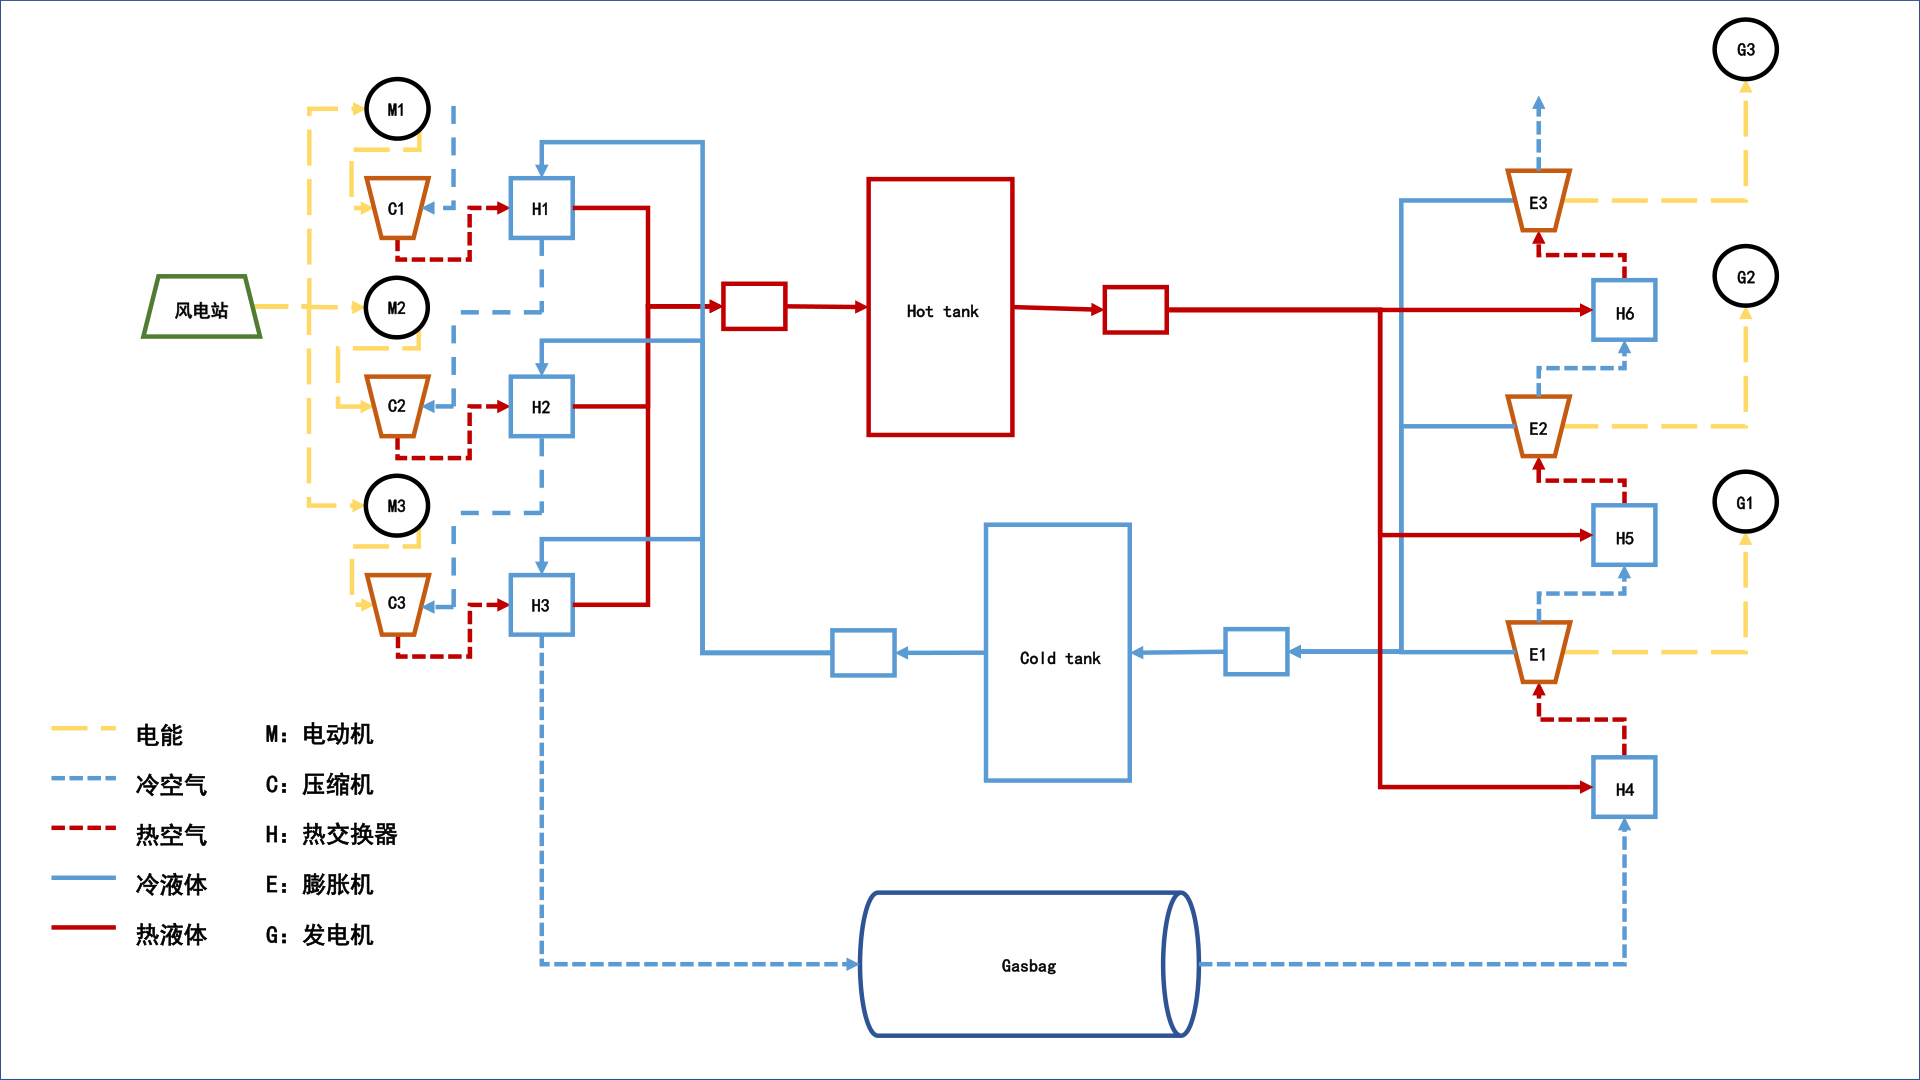
\includegraphics[scale=0.165]{pictures/The_whole_system.png}
\begin{figure}[h] %figure环境,h默认参数是可以浮动,不是固定在当前位置。如果要不浮动,你就可以使用大写float宏包的H参数,固定图片在当前位置,禁止浮动。
	\centering %使图片居中显示
	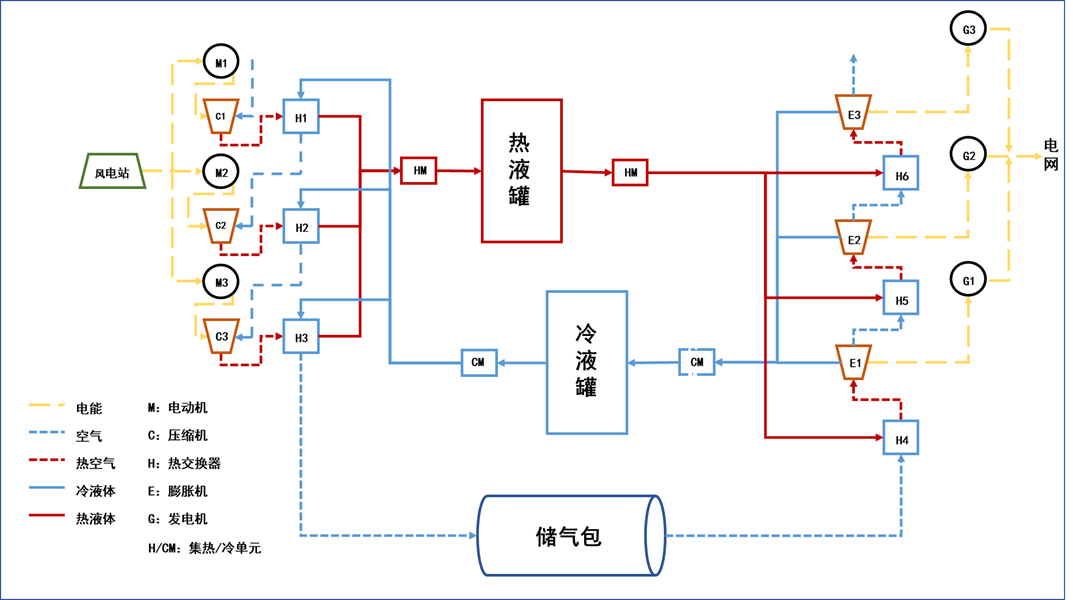
\includegraphics[width=0.8\textwidth]{pictures/screenshot001} %中括号中的参数是设置图片充满文档的大小,你也可以使用小数来缩小图片的尺寸。
	\caption{Offshore wind power generation - underwater compressed air energy storage complementary system structure diagram} %caption是用来给图片加上图题的
	\label{general system} %这是添加标签,方便在文章中引用图片。
\end{figure}%figure环境


The specific working process of the system is as follows. During energy storage, the output energy of the wind generator drives the electric motor (M1, M2, and M3) and the air compressor (C1, C2, and C3) to compress the air to a high-pressure state. A large amount of heat will be generated during the compression process. To improve compressor efficiency and reduce energy consumption, the three-stage compression and intermediate cooling method are adopted.\\

The cooling fluid (heat-conducting oil) comes from the cold liquid tank (CT), which cools the high-temperature compressed air in the heat exchangers (H1, H2, and H3), and then the hot heat-conducting fluid is collected in the hydrothermal tank (HT) for storage. Compressed air is stored in a gas storage device (GASBAG). For traditional fixed-volume compressed air energy storage, compressed air is stored in a fixed-volume gas storage device and the gas pressure in the container changes with the charging and discharging process. \\

For the complementary system of offshore wind power and underwater compressed air, the pressure of compressed air remains unchanged, while the gas storage volume in the gas storage device changes. When energy release is needed for power generation, the compressed air in the gas storage device is released, and the heat conduction liquid stored in the high-temperature heat conduction liquid storage cabinet enters the heat exchanger (H4, H5, H6) for heat exchange with the compressed air. The high-temperature and high-pressure air drive the air expander (E1, E2, E3) and the generator (G1, G2, and G3) for power generation. The air expansion device adopts three-stage expansion and intermediate heating to improve the efficiency of power generation.





\subsection{Thermodynamic model of the complementary system of offshore wind power generation and underwater compressed air energy storage}
\subsubsection{Offshore wind turbines}\ \\

\IEEEPARstart{T}{he} offshore wind turbine is the system to the nature of wind energy into electrical energy device because the wind has randomness and volatility, randomness is on the surface of the presence of the uncertainty of the wind, volatility was characterized by the size of the wind speed instability, leading to the randomness of the wind turbine output power and volatility, the presence of the uncertainty of power output and the size of the output power instability.\\

Combined with the present development of wind power generation, the offshore wind turbine model uesd in this artical is made as follow:
we used a whole month data of wind power in Gui Shan Station and fitted them. Then we cut them into 10 level, shown as \textsc{table} \ref{wind_power}, and get each probability.

%https://www.tablesgenerator.com/ 做表格用这个
% Please add the following required packages to your document preamble:
% \usepackage{booktabs}
% \usepackage{graphicx}

\begin{table}[h]
	\centering
	\resizebox{\textwidth}{!}{%
		\begin{tabular}{@{}l|llllllllll@{}}
			\toprule
			wind level & $\rho_{wind}^1$ & $\rho_{wind}^2$ & $\rho_{wind}^3$ & $\rho_{wind}^4$ & $\rho_{wind}^5$ & $\rho_{wind}^6$ & $\rho_{wind}^7$ & $\rho_{wind}^8$ & $\rho_{wind}^9$ & $\rho_{wind}^{10}$ \\ \midrule
			probability & 0.06 & 0.11 & 0.13 & 0.11 & 0.07 & 0.15 & 0.15 & 0.06 & 0.11 & 0.05 \\ \bottomrule
		\end{tabular}%
	}
	\caption{The wind level and its probability\cite{b8}}
	\label{wind_power}
\end{table}

Considering the actual situation, although the wind power is abrupt, in general, the wind power does not rise or fall substantially every 5 minutes. Therefore, the difference between two adjacent wind power levels is artificially designated to be no more than 2 in order to reflect the real situation. Figure \ref{fig:screenshot002} shows an offshore wind turbine model that is close to the real situation.


\begin{figure}[h]
	\centering
	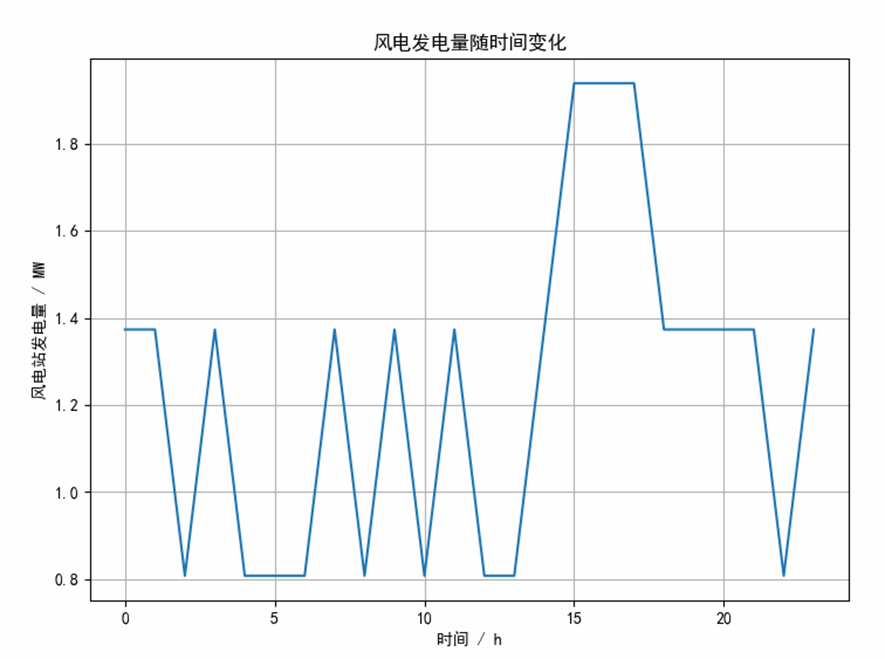
\includegraphics[width=0.7\linewidth]{pictures/screenshot002}
	\caption{Output power diagram of offshore wind turbine model}
	\label{fig:screenshot002}
\end{figure}


\subsubsection{Air compressor and air expander}\ \\\ 

\IEEEPARstart{C}{ompressor} and expander are the key points of the system. There are many kinds of compressors and expanders. In this system, centrifugal compressors and expanders are aeopt to be used.\\

The energy efficiency of the turbine is evaluated by isentropic efficiency under the assumption that all compressors have the same compression ratio and all expanders have the same expansion ratio.\\

The actual final compression temperature of the compressor is:

\begin{equation}
	T_{f, \text { comp }}=T_{\text {in }}\left[1+\frac{1}{\eta_{\text {comp }}}\left(\frac{p_{f}}{p_{i}}\right)^{\frac{r-1}{r}}\right]
	\label{f1}
\end{equation}


The actual final expansion temperature of the expander is:
\begin{equation}
T_{f, \exp }=T_{\text {in }}\left\{1-\eta_{\exp }\left[1-\left(\frac{p_{f}}{p_{i}}\right)^{\frac{r-1}{r}}\right]\right\}
\label{f2}
\end{equation}


The compression ratio of the compressor at all levels can be calculated and determined by equation \ref{f3}:

\begin{equation}
\beta_{\text {comp }}=\frac{P_{\text {out }}}{P_{\text {in }}}=\sqrt[3]{\frac{\rho g h }{P_{\text {atm }} }}
\label{f3}
\end{equation}\ 

The expansion ratio of each level of the expander can be calculated and determined by equation \ref{f4}

\begin{equation}
\beta_{\text {exp }}=\frac{P_{\text {out }}}{P_{\text {in }}}=\sqrt[3]{\frac{\rho g h }{P_{\text {atm }} }}
\label{f4}
\end{equation}\ 

The conservation of air mass in each link of the system (i.e. the trace loss of pneumatic pipeline is not taken into account) indicates that the influence of variable guide vane is not taken into account in the compressor and expander. Therefore, the actual efficiency of turbine machinery can be considered as the function of the actual flow rate and the actual compression ratio:
\begin{equation}
	\eta=f(m, \beta)
	\label{f5}
\end{equation}

The polynomial of Equation \ref{f5} can be expressed as follows:
\begin{equation}\label{f6}
	\eta_{\text {actual }}=a_{1}+a_{2} m_{\text {actual }}+a_{3} \beta_{\text {actual }}+a_{4} m_{\text {actual }} \beta_{\text {actual }}+a_{5} m_{\text {actual }}^{2}+a_{6} \beta_{\text {actual }}^{2}+a_{7} m_{\text {actual }}^{2} \beta_{\text {actual }}^{2}
\end{equation}


Assume that the rated flow rate of the compressor/expander is $ m_{rated}$,the rated compression ratio/expansion ratio is $ \beta_{rated}$,nd the rated efficiency at the design working point is $\eta_{designed}$。The dimensionless flow ratio, pressure ratio/expansion ratio, and efficiency are defined as follows:

\begin{equation}\label{f7}
	m_{n}=\frac{m_{\text {actual }}}{m_{\text {rated }}}
\end{equation}

\begin{equation}\label{f8}
	\beta_{n}=\frac{\beta_{\text {actual }}}{\beta_{\text {rated }}}
\end{equation}

\begin{equation}\label{f9}
	m_{n}=\frac{\eta_{\text {actual }}}{\eta_{\text {rated }}}
\end{equation}

Then, combined with the definitions of Equations \ref{f7} \ref{f8}  \ref{f9} and Equation \ref{f6}:

\begin{equation}\label{f10}
	\eta_{n}=b_{1}+b_{2} m_{n}+b_{3} \beta_{n}+b_{4} m_{n} \beta_{n}+b_{5} m_{n}^{2}+b_{6} \beta_{n}^{2}+b_{7} m_{n}^{2} \beta_{n}^{2}
\end{equation}

In Equation \ref{f10} ,$  \quad b_{1}=-0.03548, \quad b_{2}=0.1528811, \quad b_{3}=1.936395,b_{4}=0.1096184, \quad b_{5}=-0.1302482, \quad b_{6}=-1.0224731, \quad b_{7}=-0.0107012 $ \cite{b3}\ \\

Equation \ref{f10} is shown in Figure \ref{fig3a}:


For turbomachinery,the air pressure loss will cause the compression/expansion ratio to decrease slightly,in the system, the connector will cause this,approximately $ 0\sim 1 k P a $,far less than the air pressure, so it can be ignore. Therefore, the compression ratio and an expansion ratio of the dimensionless quantities$ \beta_{n} \approx 1 $,equation \ref{f10}can be reduced to \ref{f11}. Figure \ref{fig3a} can be converted to figure \ref{fig3b}.\\

\begin{equation}\label{f11}
	\eta_{n}=b_{1}+b_{2} m_{n}+b_{3}+b_{4} m_{n}+b_{5} m_{n}^{2}+b_{6}+b_{7} m_{n}^{2}
\end{equation}

\begin{figure}[h]
	
	\subfigure[is the enthalpy of air, which can be calculated by Equation ] %第一张子图
	{
		\begin{minipage}{0.5\linewidth}
			\centering          %子图居中
			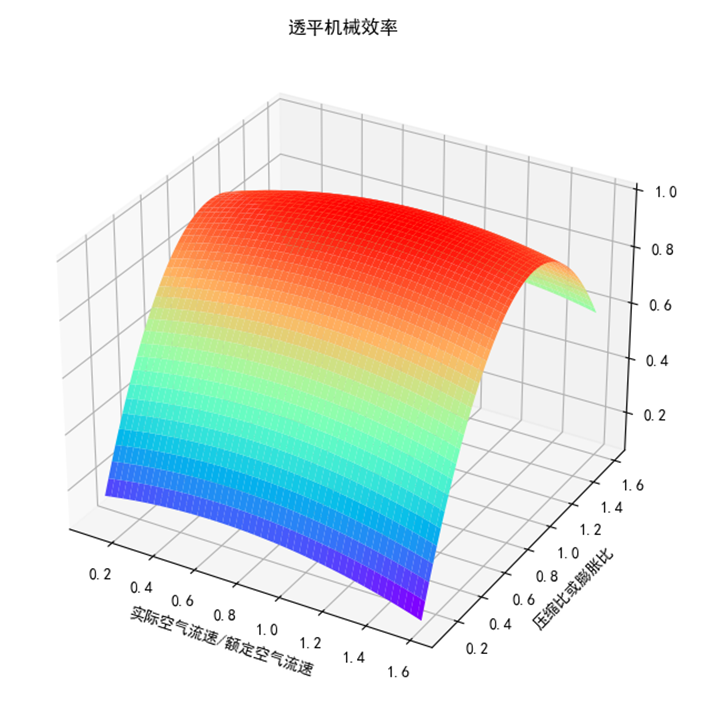
\includegraphics[width=0.9\linewidth]{pictures/screenshot003}
			\label{fig3a}   %以pic.jpg的0.5倍大小输出
		\end{minipage}
	}
	\subfigure[Dimensionless relation diagram of typical turbine mechanical efficiency and air mass flow] %第二张子图
	{
		\begin{minipage}{0.5\linewidth}\label{b}
			\centering      %子图居中
			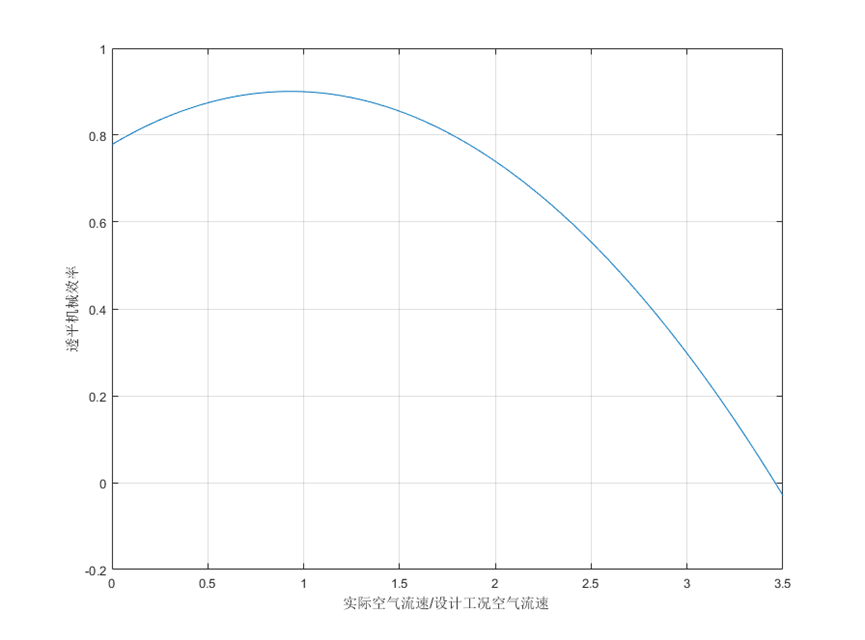
\includegraphics[width=0.9\linewidth]{pictures/screenshot004}
			\label{fig3b}   %以pic.jpg的0.5倍大小输出
		\end{minipage}
	}
	
	
	\caption{Equation \ref{f10} and equation \ref{f11}} %  %大图名称
	\label{fig:3}  %图片引用标记
\end{figure}

The compression power/expansion power of the compressor/expander for air can be calculated according to Equation \ref{f12} :
\begin{equation}\label{f12}
	P_{\text {comp }}=m_{\text {compressor }}\left(H_{\text {out }}-H_{\text {in }}\right) P_{\text {expander }}=m_{\text {expander,air }}\left(H_{\text {in }}-H_{\text {out }}\right)
\end{equation}

$ H $ is the enthalpy of air, which can be calculated by Equation \ref{f13} :

\begin{equation}\label{f13}
	H_{a i r}=4.6020+0.9705 T+3.3955 \times 10^{-5} T^{2}+3.3955 \times 10^{-8} T^{3}+1.697 \times 10^{-11} T^{4}
\end{equation}



\subsubsection{Heat exchange system}\ \\

\IEEEPARstart{T}{he} heat exchange system is composed of a heat exchanger and heat storage unit (divided into small units and heat storage tank). In this system, the heat exchanger is the core equipment connecting the compression subsystem and the expension subsystem. \\

The performance of the heat exchanger is usually measured by the efficiency, which is defined as the ratio of the actual heat transfer and the maximum possible heat transfer:\\

\begin{equation}\label{f14}
	\epsilon=\frac{\dot{Q}_{actual}}{\dot{Q}_{max}}=\frac{(\dot{m}c_p\Delta T)_{cold \  or \  hot}}{(\dot{m}c_p)_{min}(T_{hot,in}-T_{cold,in})}
\end{equation}

$ \left(\dot{m}{c_{p}}\right)_{\min } $ represents the smaller of the hot fusion rate of hot fluid and cold fluid.\\

In this system, using $ \epsilon=0.9 $。\\

Hypothesis one of the air compression work $ W_{\text {comp},i}(i=1,2,3) $, increase the air $ \Delta Q_{\text {comp}, i}(i=1,2,3) $, then after with low-temperature heat conduction oil heat transfer in the heat exchanger, air temperature can be calculated by equetion \ref{f15} :
\begin{equation}\label{f15}
	c_{a i r} m_{a i r}\left(T_{i n, a i r}-T_{o u t, a i r}\right)=\epsilon \Delta Q_{c o m p, i}(i=1,2,3)
\end{equation}

$ c_{a i r} $ is the specific heat capacity of air, which can be calculated by Equation \ref{f16}:

\begin{equation}\label{f16}
	c_{a i r}=0.9705+6.791 \times 10^{-5} T+1.658 \times 10^{-7} T^{2}-6.788 \times 10^{-11} T^{3}
\end{equation}

Heat conduction oil absorbs heat and is stored in a heat storage tank through a small heat storage unit. The heat storage tank is built with thermal insulation materials, and therefore, the heat loss can be ignored. The heat-conducting oil in the heat storage tank can be calculated by Equation \ref{f17}:

\begin{equation}\label{f17}
	\sum \epsilon \Delta Q_{\text {comp },i}=c_{\text {oil }} m_{\text {oil }}\left(T_{\text {out }, \text { oil }}-T_{\text {in,oil }}\right)(i=1,2,3)
\end{equation}

$ c_{\text {oil }} $ is the specific heat capacity of heat conducting oil, which can be calculated by Equation \ref{f18}:
\begin{equation}\label{f18}
	c_{o i l}=1.2266+0.0014(T-273.15)
\end{equation}

For the heat exchanger connected to the expander, the air temperature can be calculated by Equation \ref{f19}:

\begin{equation}\label{f19}
	T_{\text {air,hot }}=T_{\text {air,cold }}+\epsilon \frac{\left(\dot{m} c_{p}\right)_{\min }}{\left(\dot{m} c_{p}\right)_{\text {air }}}\left(T_{\text {oil,hot }}-T_{\text {air,cold }}\right)
\end{equation}

After heat exchanging, the cold heat conducting oil flow into the cold liquid tank. The cold liquid tank is constructed of materials with good thermal conductivity. The temperature of the cold liquid tank can be kept the same as that of the sea area where it is located, $ 290K $\ \\


\subsubsection{Gas storage device}
\ \\

\IEEEPARstart{T}{he} function of the air storage device is to store compressed air generated by conp. This system plans to use the spherical flexible gas storage device to realize the constant pressure storage of compressed air by using the static pressure characteristics of water. The temperature and pressure of the compressed air in the gas storage device are the same as the temperature and pressure of the water body.\\


The temperature of compressed air can be calculated by Equation \ref{f20} :

\begin{equation}
	T_{gasbag}=T_{water}
	\label{f20}
\end{equation}

The pressure of compressed air can be calculated by Equation \ref{f21}:
\begin{equation}
	P_{air,gasbag}=P_{water}=\rho_{water}gh
	\label{f21}
\end{equation}

\subsubsection{Motor and generator}
\ \\

\IEEEPARstart{A}{s} shown in Figure \ref{general system}, there are three motors and three generators in the system.\\

Taking one motor and one generator as an example:\\

The power generation:
\begin{equation}
	W_{\text {generator},i}=\eta_{\text {generator }} W_{\text {expander},i}(i=1,2,3)
	\label{f23}
\end{equation}

$ \eta_{\text {generator }} $ is the generating efficiency of $ G1,G2,G3 $, and the $ \eta_{\text {generator }} $ is tentatively determined to be $ \eta_{\text {generator }} =95\%$\\

The power consumption:

\begin{equation}
	W_{\text {motor }}=c_{i} W_{\text {wind }}(i=1,2,3)
	\label{f22}
\end{equation}



$ c_i  $ is the proportion of wind power distribution, and  tentatively determines $ c_{1}=32.24 \%, \quad c_{2}=33.06 \%, \quad c_{3}=34.7 \% $\\ 



The total power consumed by the system motor and the total power generated by the generator can be calculated by Equations \ref{f24} and \ref{f25}:

\begin{equation}
	W_{motor,total}=W_{motor,1}+W_{motorr,2}+W_{motor,3}
	\label{f24}
\end{equation}
\begin{equation}
	W_{generator,total}=W_{generator,1}+W_{generator,2}+W_{generator,3}
	\label{f25}
\end{equation}



\section{Solving the thermodynamic model of the system}

\IEEEPARstart{T}{he} operation of the complementary energy storage system of offshore wind power generation and underwater compressed air can be divided into four basic working processes: offshore wind power generation process, compression energy storage process, storage process, and expansion energy release process.\\

Offshore wind turbines convert wind energy into electricity to drive electric motors that drive compressors to store compressed air and high-temperature heat conductors. In the process of energy release, the stored compressed air is released to drive the expander and generator, and the heat energy stored in the heat-conducting liquid is released at the same time. \\

The basic parameters of the system are shown in Table \ref{tab:my-table}

\begin{table}[h]
	\centering
	\resizebox{\textwidth}{!}{
	\begin{tabular}{l|c|r|l|c|r}
		\multicolumn{1}{c|}{Parameter} & Unit                      & \multicolumn{1}{c}{Reference Value} &\multicolumn{1}{|c|}{Parameter} & Unit                     & \multicolumn{1}{c}{Reference Value} \\ \hline
		                    &                     &                      &                 &                       & \\
		atmospheric pressure                    & Pa                      & 101325                      &Total time of expansion potential energy                 & hour                      & 3\\
		Atmospheric temperature                   & K                       & 298.15                      &Rated isentropic efficiency of expander 1              & \%                      & 90 \\
		Rated air flow rate                 & kg/s                    & 8.5                         &Rated isentropic efficiency of expander 2              & \%                      & 90\\
		Rated output power of wind power plant              & MW                      & 2.45                        &Rated isentropic efficiency of expander 3              & \%                      & 90\\
		Rated input efficiency of motor M1
		
		             & \%                      & 90                          &Rated expansion ratio of expander 1
		             
		                            &                         & 2.1544\\
		Rated input efficiency of motor M2
		
		            & \%                      & 90                          &Rated expansion ratio of expander 2
		            
		                           &                         & 2.1544\\
		Rated input efficiency of motor M1
		
		            & \%                      & 90                         &Rated expansion ratio of expander 3
		            
		                           &                         & 2.1544 \\
		Motor M1 rated input power             & MW                      & 0.79                        &Expansion power of expander 1                & MW                      & 1.76 \\
		Motor M2 rated input power             & MW                      & 0.81                        &Expansion power of expander 2                & MW                      & 1.77\\
		Motor M3 rated input power             & MW                      & 0.84                        &Expansion power of expander 3                & MW                      & 1.77\\
		Rated isentropic efficiency of compressor 1              & \%                      & 90                          &Rated generation efficiency of generator 1              & \%                      & 95\\
		Rated isentropic efficiency of compressor 2              & \%                      & 90                         &Rated generation efficiency of generator 2              & \%                      & 95\\
		Rated isentropic efficiency of compressor 3              & \%                      & 90                          &Rated generation efficiency of generator 3              & \%                      & 95\\
		Compressor 1 rated equal compression ratio              &                         & 2.1544                     &Rated output power of generator 1              & MW                      & 1.67 \\
		Compressor 2 rated equal compression ratio             &                         & 2.1544                      &Rated output power of generator 2              & MW                      & 1.68\\
		Compressor 3 rated equal compression ratio              &                         & 2.1544                      &Rated output power of generator 3              & MW                      & 1.68\\
		Total time of compressed energy storage                 & H                       & 9                         &Rated efficiency of heat exchanger                &                         & 0.9  \\
		Rated underwater storage depth                & m                       & 100                        &Rated heat exchange power of heat exchanger 1              & MW                      & 0.64  \\
		Storage pressure                    & Pa                      & 1013201                    &Rated heat exchange power of heat exchanger 2              & MW                      & 0.68 \\
		Total mass of stored air                 & kg                      & 275400                      &Rated heat exchange power of heat exchanger 3              & MW                      & 0.68\\
		Rated air density                  & $ kg/m^3 $ & 11                         &Rated heat exchange power of heat exchanger 4              & MW                      & 2.27 \\
		Total volume of stored air                 & $ m^3  $   & 25036.4                    &Rated heat exchange power of heat exchanger 5              & MW                      & 1.81 \\
		Specification of gasbag                   & $ m^3 $    & 30000                      &Rated heat exchange power of heat exchanger 6              & MW                      & 1.77  \\
		Storage time                   & hour                      & 3                          &Heat transfer oil flow rate \& air flow rate          & kg/s                    & 1.7  \\
		Rated expansion air flow rate                & kg/s                    & 25.5                        &Heat transfer oil flow rate \& air flow rate           & kg/s                    & 1.7  \\
		Rated temperature of heat storage tank                 & K                       & 388                         &System cycle efficiency                  & \%                      & 68.46\\
		Rated temperature of coolant tank                 & K                       & 290                         
		                      
	\end{tabular}
}
	\caption{Relevant parameters of the system under rated operating conditions}
	\label{tab:my-table}
\end{table}

The total energy consumption in the process of compressed energy storage can be calculated by Equation \ref{f31}:
\begin{equation}\label{f31}
	W_{\text {motor,total }}=W_{\text {motor }, 1}+W_{\text {motorr }, 2}+W_{\text {motor }, 3}=\int_{0}^{t_{1}}\left(P_{m 1}+P_{m 2}+P_{m 3}\right) d t
\end{equation}


$ t_1 $ is the time consumed by compressed air.\\

The total electric energy produced in the expansion energy release process can be calculated by Equation \ref{f32}:
\begin{equation}\label{f32}
	W_{\text {generator,total }}=W_{\text {generator, } 1}+W_{\text {generator, } 2}+W_{\text {generator }, 3}=\int_{0}^{t_{2}}\left(P_{G 1}+P_{G 2}+P_{G 3}\right) d t
\end{equation}

$ t_2 $ is the time consumed by releasing energy\\

System efficiency can be calculated by Equation \ref{f33}:


\begin{equation}\label{f33}
		\begin{aligned}
		\eta_{\text {system }}&=\frac{W_{\text {generator,total }}}{W_{\text {motor,total }}}=\frac{\int_{0}^{t_{2}}\left(P_{G 1}+P_{G 2}+P_{G 3}\right) d t}{\int_{0}^{t_{1}}\left(P_{m 1}+P_{m 2}+P_{m 3}\right) d t}
		\\
		&=\frac{\int_{0}^{t_{2}} \eta_{\text {generator }}\left(P_{\text {expander } 1}+P_{\text {expander } 2}+P_{\text {expanders }}\right) d t}{\int_{0}^{t_{1}}\left(P_{\text {wind }}\right) d t}\\
		&=\frac{\int_{0}^{t_{2}} \eta_{\text {generator }}\left(m_{\text {expander,air} }(H_{in,4}-H_{out,4})+m_{\text {expander,air} }(H_{in,5}-H_{out,5})+m_{\text {expander,air} }(H_{in,6}-H_{out,6})\right) d t}{\int_{0}^{t_{1}}\left(P_{\text {wind }}\right) d t}
	\end{aligned}
\end{equation}


Because $\int_{0}^{t_{2}} m_{\text {expander,air }}=\int_{0}^{t_{1}} m_{\text {compressor, air }}  $, Equation \ref{f33} can be transformed into Equation \ref{f34}:

\begin{equation}\label{f34}
	\begin{aligned}
		\eta_{\text {system }}&=\frac{\left(\left(H_{\text {in,expander } 1}-H_{\text {out } 4, \text { expander } 1}\right)+\left(H_{\text {in, expander } 2}-H_{\text {out,expander } 2}\right)+\left(H_{\text {in,expander } 3}-H_{\text {out,expander3 }}\right)\right) }{\int_{0}^{t_{1}}\left(P_{\text {wind }}\right) d t}\\ 
		&\times \eta_{\text {generator }} \int_{0}^{t_{1}} m_{\text {compressor,air}} d t
	\end{aligned}
\end{equation}

The air flow in expension subsystrem $ m_{\text {expander, air }} $ can be fixed in a certain stavle value. Therefore, \\
$ \left(H_{\text {in,expander } 1}-H_{\text {out } 4, \text { expander } 1}\right)+\left(H_{\text {in, expander } 2}-H_{\text {out,expander } 2}\right)+\left(H_{\text {in,expander } 3}-H_{\text {out,expander3 }}\right) $ can be approximately considered as a fixed valueThe, enthalpy difference can be approximated as a fixed value.\\

根据式\ref{f13}:焓差是关于温差的函数,所以该焓差与膨胀机1,2,3的膨胀终温和换热器4,5,6的出口温度之差有关。首先讨论与膨胀终温有关的因素,根据式\ref{f2},膨胀终温与膨胀比和膨胀效率有关,图\ref{fig4a}所示为膨胀比和膨胀效率与膨胀机膨胀终温的关系;因为气动管路压力损失可忽略不计,故膨胀比近似额定膨胀比,膨胀机出口温度与入口温度比值如图\ref{fig4b}所示可近似关于膨胀机效率的一次函数。由图\ref{fig4b}可知,膨胀机膨胀效率越大,膨胀机出入口温度比值越小。其次讨论与换热器4,5,6出口温度有关的因素,根据式\ref{f19},换热器4,5,6出口温度与高温导热油的温度成正比,根据式\ref{f17},可得式\ref{f35}:

\begin{figure}[ht]
	\subfigure[Expander inlet and outlet temperature ratio, expansion ratio and expansion efficiency] %第一张子图
	{
		\begin{minipage}{0.5\linewidth}
			\centering          %子图居中
			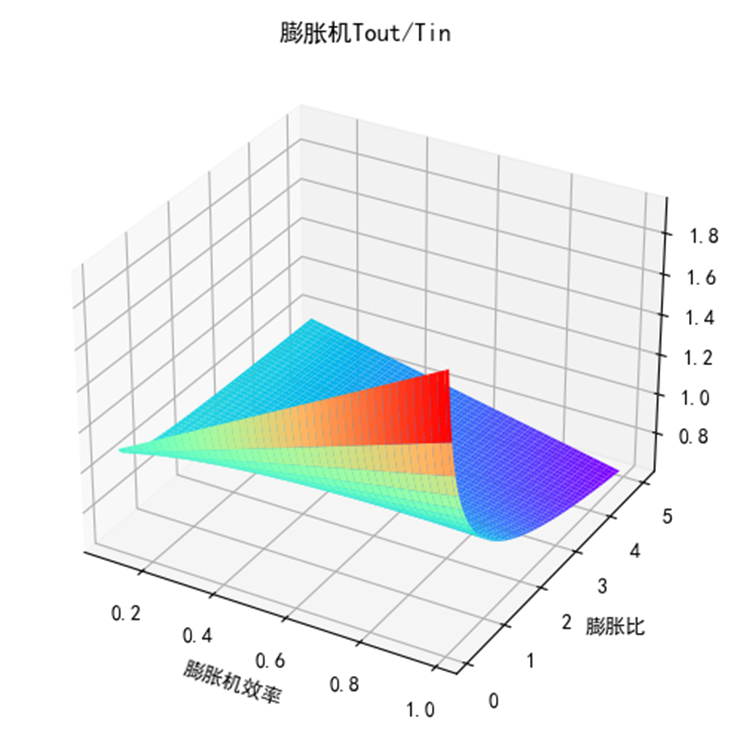
\includegraphics[width=0.9\linewidth]{pictures/screenshot005}
			\label{fig4a}   %以pic.jpg的0.5倍大小输出
		\end{minipage}
	}
	\subfigure[Relationship between Expander Inlet and Outlet Temperature Ratio and Expander Efficiency((Ignored Small Changes in Expander Ratio)] %第一张子图
{
	\begin{minipage}{0.5\linewidth}
		\centering          %子图居中
		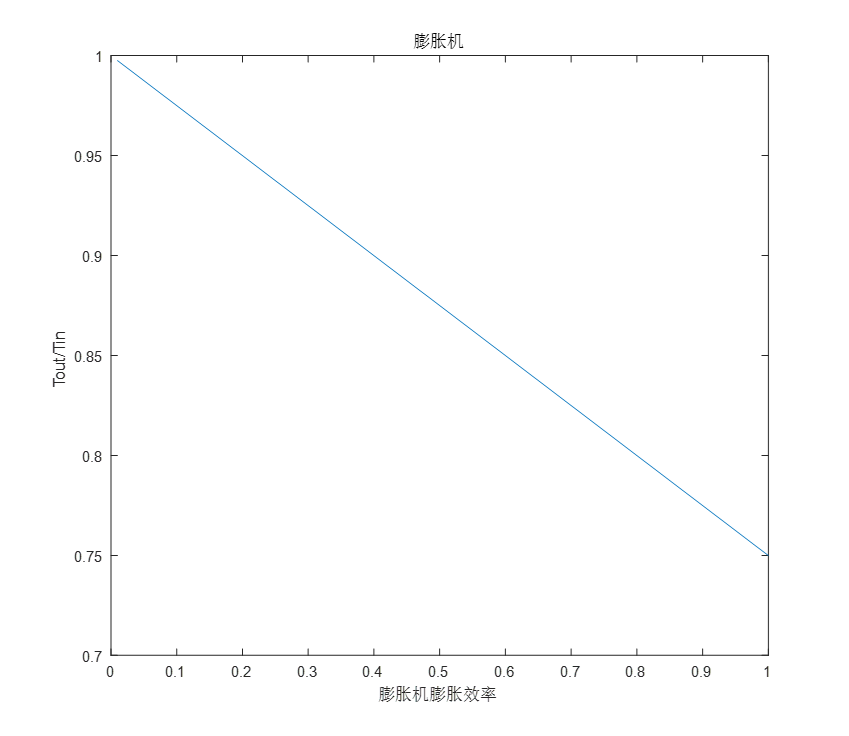
\includegraphics[width=0.9\linewidth]{pictures/screenshot006}
		\label{fig4b}   %以pic.jpg的0.5倍大小输出
	\end{minipage}
}
	\subfigure[Compressor inlet and outlet temperature ratio and compression ratio and compression efficiency] %第一张子图
{
	\begin{minipage}{0.5\linewidth}
		\centering          %子图居中
		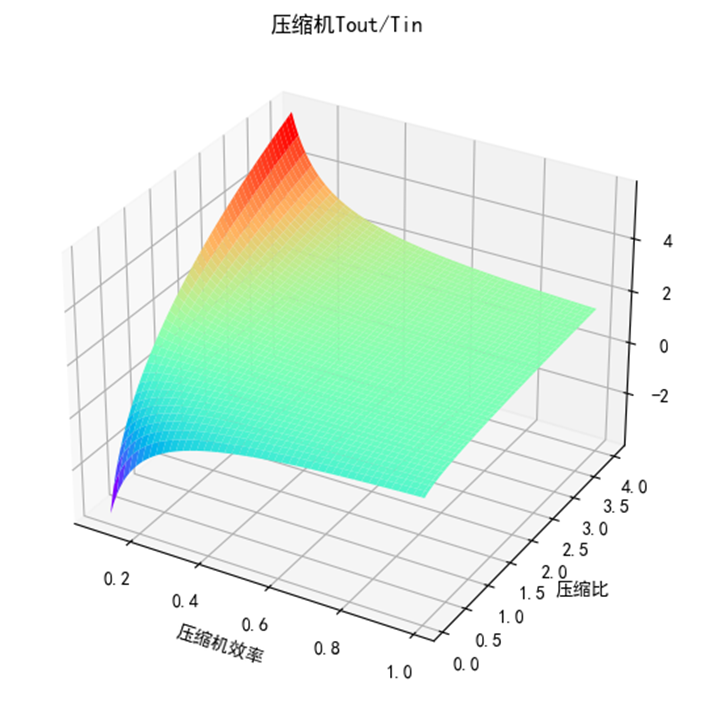
\includegraphics[width=0.9\linewidth]{pictures/screenshot007}
		\label{fig4c}   %以pic.jpg的0.5倍大小输出
	\end{minipage}
}
	\subfigure[Relation between compressor inlet and outlet temperature ratio and compression efficiency (ignoring the slight change of compression ratio)] %第一张子图
{
	\begin{minipage}{0.5\linewidth}
		\centering          %子图居中
		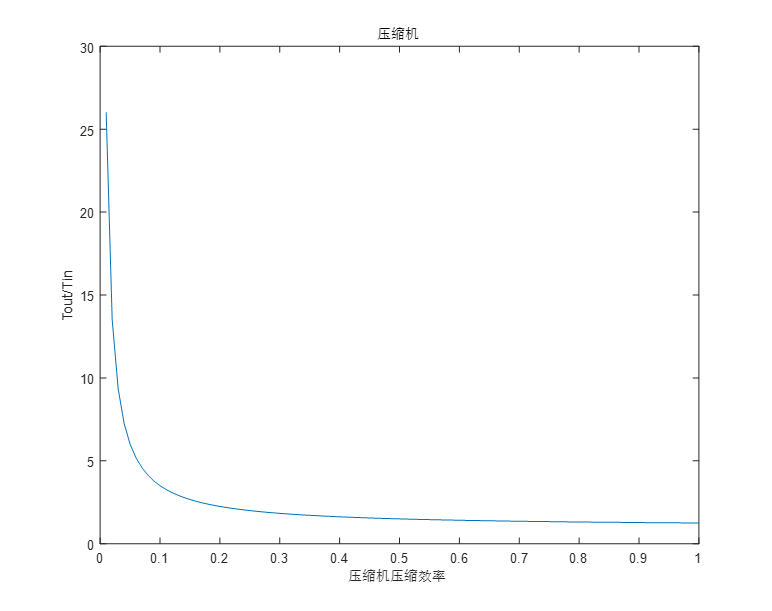
\includegraphics[width=0.9\linewidth]{pictures/screenshot008}
		\label{fig4d}   %以pic.jpg的0.5倍大小输出
	\end{minipage}
}
	\caption{Efficiency in compressor and expander} %  %大图名称
\label{fig:4}  %图片引用标记

\end{figure}
\begin{equation}\label{f35}
	\begin{aligned}
		&T_{\text {out,oil }}=T_{\text {in,oil }}+\epsilon \cdot m_{\text {compressor, air }}\\
		&\times \frac{\left(H_{\text {out }, \text { compressor } 1}-H_{\text {in, compressor } 1}\right)+\left(H_{\text {out }, \text { compressor } 2}-H_{\text {in, compressor } 2}\right)+\left(H_{\text {out, } \text { compressor } 3}-H_{\text {in, compressor } 3}\right)}{m_{\text {oil }}}
	\end{aligned}
\end{equation}

可见,高温导热油的温度与$ \frac{m_{\text {compressor,air }}}{m_{\text {oil }}} $和$\left(H_{\text {out }, \text { compressor } 1}-H_{\text {in, compressor } 1}\right)+\left(H_{\text {out }, \text { compressor } 2}-H_{\text {in, compressor } 2}\right)$\\

$+\left(H_{\text {out, } \text { compressor } 3}-H_{\text {in, compressor } 3}\right)  $有关。\\

其中:与$ \frac{m_{\text {compressor,air }}}{m_{\text {oil }}} $越大,$ T_{\text {out }, \text { oil }} $越大。\\

$\left(H_{\text {out }, \text { compressor } 1}-H_{\text {in, compressor } 1}\right)+\left(H_{\text {out }, \text { compressor } 2}-H_{\text {in, compressor } 2}\right)+\left(H_{\text {out, } \text { compressor } 3}-H_{\text {in, compressor } 3}\right)  $与压缩机的压缩比和压缩效率有关,图\ref{fig4c}所示为压缩比和压缩效率与压缩机压缩终温的关系;因为气动管路压力损失可忽略不计,故压缩比近似额定压缩比,压缩机出口温度和入口温度的比值如图\ref{fig4d}所示可近似于压缩机效率的反比例型函数。由图\ref{fig4d}可知,压缩机出入口温度比值与压缩效率成反比。

In summary, the main factors affecting the efficiency of the complementary energy storage system of offshore wind power generation and underwater compressed air are as follows:
\begin{enumerate}
	\item compression ratio and compression efficiency
	\item expansion ratio and expansion efficiency
	\item the output power of the wind power station
	\item the ratio of air mass flow rate and oil mass flow rate in the compression process, $ \frac{m_{\text {compressor,air }}}{m_{\text {oil }}} $
\end{enumerate}

In order to improve the system efficiency, we can improve the compression ratio, compression efficiency, and also $ \frac{m_{\text {compressor,air }}}{m_{\text {oil }}} $. Usually, we umcrease the compression ratio. 

\section{Operating characteristics of the complementary system of OWPG-UCAES system under different working conditions}
\ \\

通常系统运行工况可以分为额定设计工况和非设计工况两种。设计下系统性能是比较优越的,系统各组件通常工作在设计工况点,储存的能量利用率也通常较高,所以系统效率也是较高的。因此,通常希望系统能够保持在设计工况点或设计工况点附近运行,从而获得最佳的系统效率和工作性能。但是,在某些情况下系统会不可避免地工作在非设计工况,这在供能和负荷波动的储能系统中表现得尤为突出。对于这类非设计工况工作比例很大的系统而言,研究其非设计工况系统特性对系统的设计优化是十分重要和有必要的。本小节研究水下压缩空气储能系统在设计工况和非设计工况下的运行特性,并进行对比分析。

\subsection{Operation of the system under design conditions}

A complete operation cycle of the system design condition includes:
\begin{enumerate}
	\item Energy storage: the compression energy storage device runs under the design condition to complete the complete inflation of the gas storage device
	\item Storage: energy storage process 
	\item Energy release: the expansion power generation equipment runs under the design condition to completely release the compressed air in the gas storage device
\end{enumerate}

The basic parameters of the system are taken as reference in table \ref{tab:my-table}. It is tentatively determined that the compression energy storage stage will last for about 9 hours in a cycle, follow by 3 hours of energy storage process, and the energy release process will also last for 3 hours.The duration of the energy release process is far less than the duration of energy storage because the generated power is far more than the power consumption, and the system cycle efficiency is inevitably less than 于100\%. Besides, the little pressre lost in the connection in this system is ingored. 

\begin{figure}[ht]
	\subfigure[系统设计工况条件下运行一周期的储气装置内压缩空气总质量变化] %第一张子图
	{
		\begin{minipage}{0.5\linewidth}
			\centering          %子图居中
			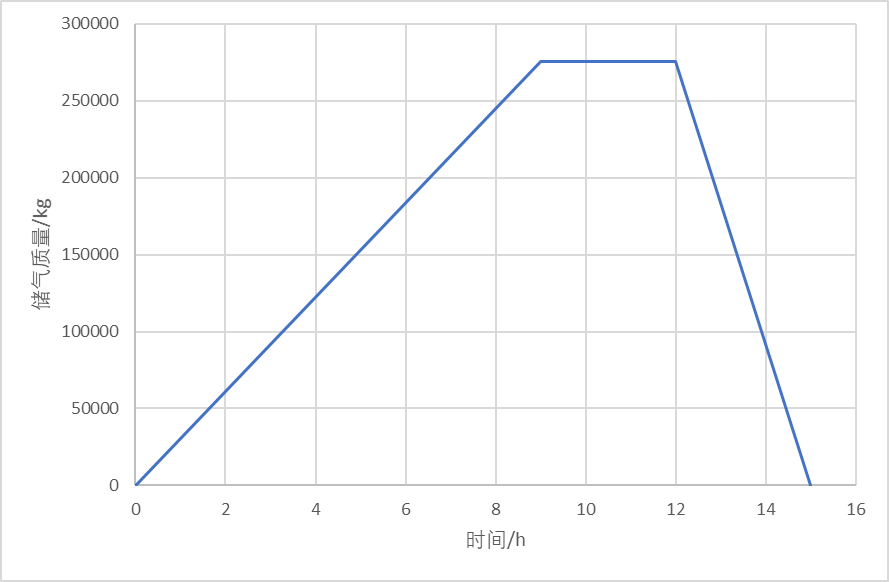
\includegraphics[width=0.9\linewidth]{pictures/screenshot009}
			\label{fig5a}   %以pic.jpg的0.5倍大小输出
		\end{minipage}
	}
	\subfigure[系统设计工况条件下运行一周期的储气装置内压缩空气总体积变化] %第一张子图
	{
		\begin{minipage}{0.5\linewidth}
			\centering          %子图居中
			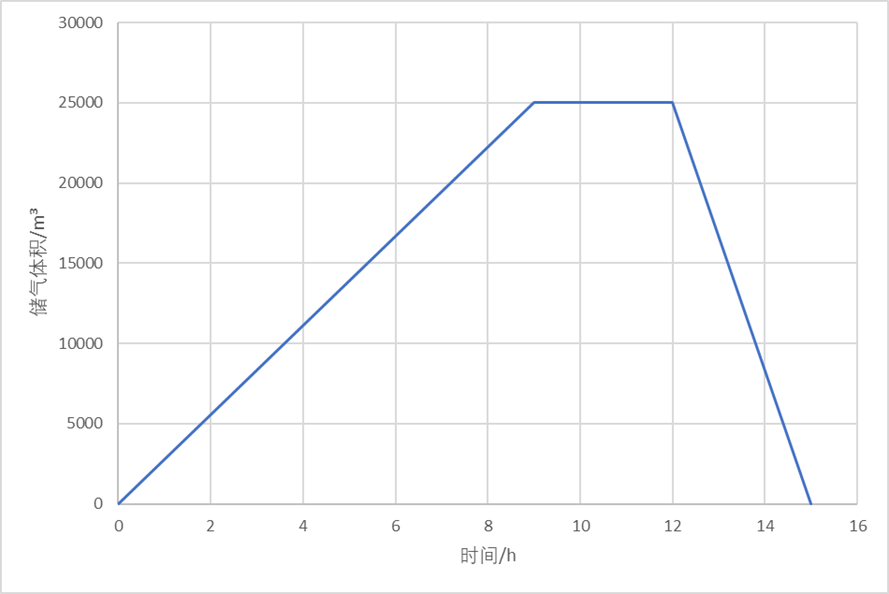
\includegraphics[width=0.9\linewidth]{pictures/screenshot010}
			\label{fig5b}   %以pic.jpg的0.5倍大小输出
		\end{minipage}
	}
	\caption{额定工况下储气包的变化} %  %大图名称
	\label{fig:5}  %图片引用标记
\end{figure}
 
Figure \ref{fig5a} and figure \ref{fig5b} respectively system running a cycle in the design operating conditions of the total quality of compressed air in a gas storage device and the change of total volume,   it can be seen that the gas loss compared to the gas storage capacity of a gas storage device is very small, even negligible, in other words, the system of natural discharge rate is negligible, it is also an offshore wind power - underwater complementary compressed air energy storage system can be used as the energy storage system for a long time.

\begin{figure}[ht]
	\subfigure[系统设计工况条件下运行一周期电动机输入功率和发电机的输出功率变化] %第一张子图
	{
		\begin{minipage}{0.5\linewidth}
			\centering          %子图居中
			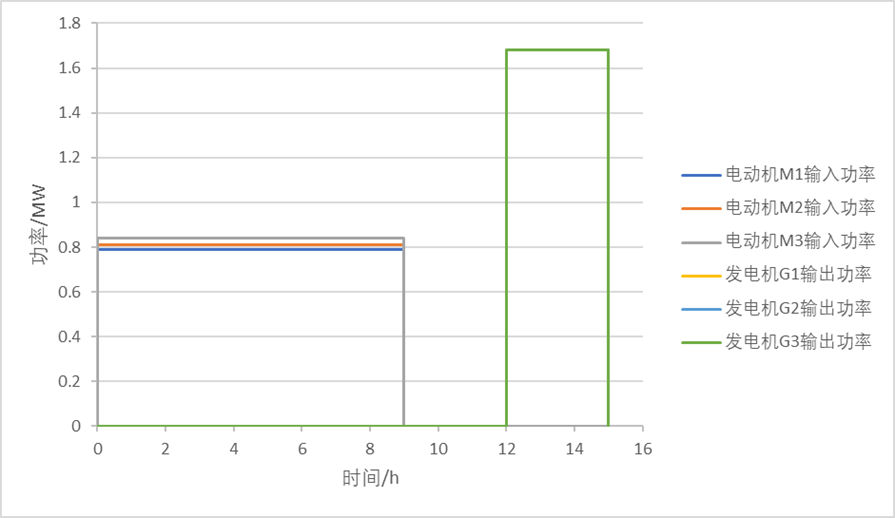
\includegraphics[width=0.9\linewidth]{pictures/screenshot011}
			\label{fig6a}   %以pic.jpg的0.5倍大小输出
		\end{minipage}
	}
	\subfigure[系统设计工况条件下运行一周期空气压缩机压缩效率和空气膨胀机膨胀效率变化] %第一张子图
	{
		\begin{minipage}{0.5\linewidth}
			\centering          %子图居中
			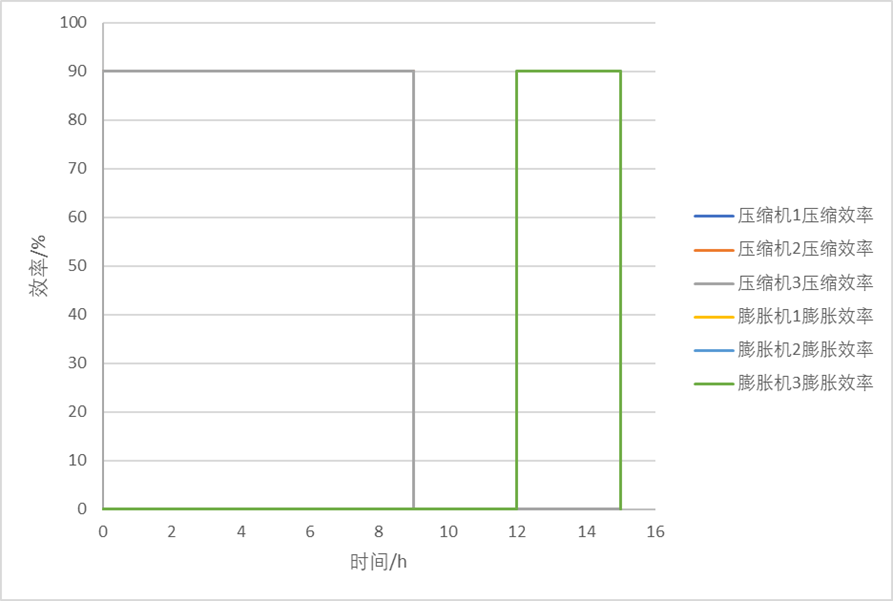
\includegraphics[width=0.9\linewidth]{pictures/screenshot012}
			\label{fig6b}   %以pic.jpg的0.5倍大小输出
		\end{minipage}
	}
	\subfigure[系统设计工况条件下运行一周期高温导热油和低温导热油的质量变化] %第一张子图
	{
		\begin{minipage}{0.5\linewidth}
			\centering          %子图居中
			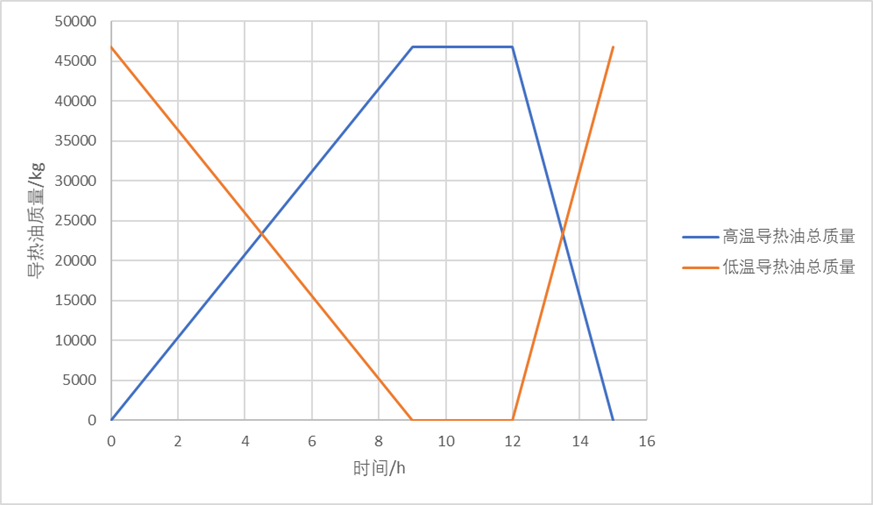
\includegraphics[width=0.9\linewidth]{pictures/screenshot013}
			\label{fig6c}   %以pic.jpg的0.5倍大小输出
		\end{minipage}
	}
	\subfigure[系统设计工况条件下运行一周期系统效率变化] %第一张子图
	{
		\begin{minipage}{0.5\linewidth}
			\centering          %子图居中
			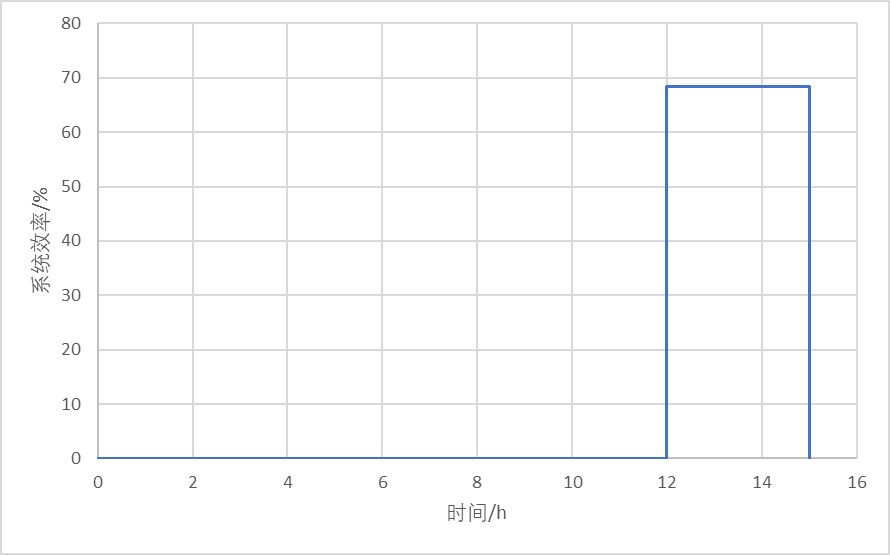
\includegraphics[width=0.9\linewidth]{pictures/screenshot014}
			\label{fig6d}   %以pic.jpg的0.5倍大小输出
		\end{minipage}
	}
	\caption{系统设计工况条件下各系统运行情况} %  %大图名称
	\label{fig:6}  %图片引用标记
\end{figure}

Figure \ref{fig6a} shows the variation of the input power of the motor that drives the air compressor and the output power of the generator connected to the air expander during one cycle of operation under the design condition of the system. It can be seen that the power of the motor/generator is stable.\\

Figrue \ref{fig6b} shows the variation of the compression efficiency of the air compressor and the expansion efficiency of the air expander during one cycle of operation of the system under the design working conditions. Because the compressor and the expander work under the design working conditions, both the compressor and the expander work at the rated efficiency.\\

Figure \ref{fig6c} shows the quality changes of high-temperature and low-temperature heat transfer oil during one cycle of system operation under design working conditions. Because the high-temperature and low-temperature heat transfer oil circulate steadily under design working conditions, the quality change curves of the two are symmetrical.\\

图\ref{fig6d}所示为系统在设计工况条件下运行一周期的系统效率变化,其表现在膨胀释能过程,设计工况条件下系统效率可达68.46\%,相比于火力发电厂,水力发电厂,风力发电站等常规发电机构的系统效率而言,系统效率有了极大的提高。

\subsection{系统变工况运行}
\subsubsection{系统变工况分析思路}\ \\

根据3节的热力学模型分析,假设本系统压缩储能过程工作在变工况条件,膨胀释能过程因受控程度比压缩储能过程更高,故膨胀释能过程工作在设计工况条件。以下是压缩储能过程在变工况条件下运行的分析思路。\\


首先,海上风力发电机组输出功率随海上风速变化而变化的电能,其输出功率范围为$ [0MW,3.06MW] $,电动机$ M1,M2,M3 $分别以$ 32.24\%,33.06\% $和$ 34.7\% $的比例将海上风力发电机组的输出电能划分,如图\ref{fig7a}所示为海上风力发电机组实际输出功率与各台电动机实际输入功率的关系图,由表\ref{tab:my-table}可知,海上风力发电机组在额定工况条件下的输出值为$ 2.45MW $,电动机$ M1,M2 $和$ M3 $在额定工况条件下的输入值分别为$ 0.79MW,0.81MW $和$ 0.84MW $,以这些数值为基准值,可以得到如图\ref{fig7b}所示的海上风力发电机组输出标幺值与各台电动机输入标幺值关系图。

\begin{figure}[ht]
	\subfigure[海上风力发电机组实际输出功率与各台电动机实际输入功率的关系] %第一张子图
	{
		\begin{minipage}{0.5\linewidth}
			\centering          %子图居中
			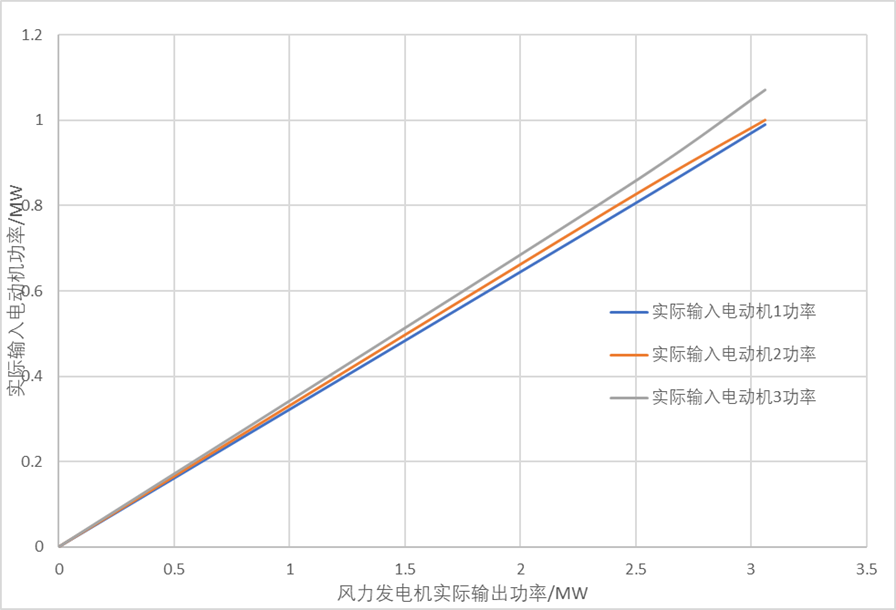
\includegraphics[width=0.9\linewidth]{pictures/screenshot015}
			\label{fig7a}   %以pic.jpg的0.5倍大小输出
		\end{minipage}
	}
	\subfigure[海上风力发电机组输出标幺值与各台电动机输入标幺值关系] %第一张子图
	{
		\begin{minipage}{0.5\linewidth}
			\centering          %子图居中
			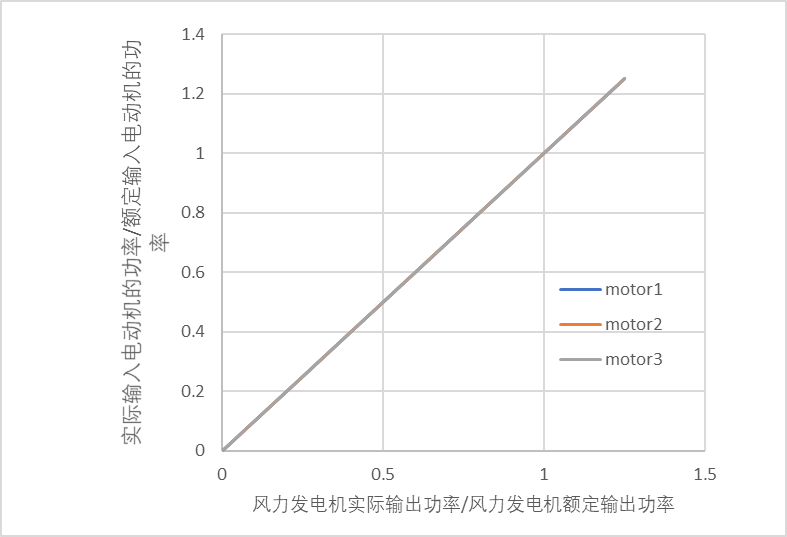
\includegraphics[width=0.9\linewidth]{pictures/screenshot016}
			\label{fig7b}   %以pic.jpg的0.5倍大小输出
		\end{minipage}
	}
	\caption{变工况下电动机的输入} %  %大图名称
	\label{fig:7}  %图片引用标记
\end{figure}

其次,电动机$ M1.M2 $和$ M3 $分别驱动空气压缩机$ C1,C2 $和$ C3 $对空气进行压缩,当电动机实际输入功率变化时,进入空气压缩机的空气质量流量也随之变化,如图\ref{fig:screenshot017}所示为电动机输入功率标幺值与空气质量流量标幺值(以$ 8.5kg/s $为基准值)的关系图。

\begin{figure}[h]
	\centering
	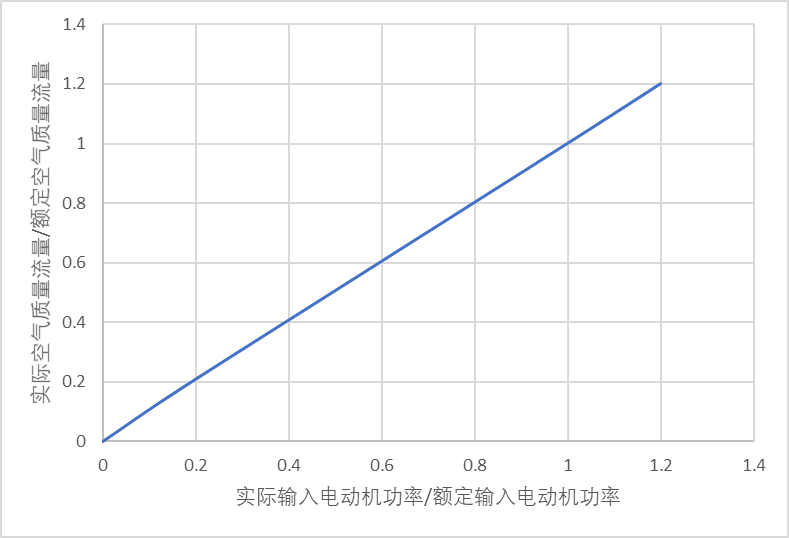
\includegraphics[width=0.7\linewidth]{pictures/screenshot017}
	\caption{电动机输入功率标幺值与空气质量流量标幺值(以$ 8.5kg/s $为基准值)的关系图}
	\label{fig:screenshot017}
\end{figure}

再次,当进入空气压缩机空气质量流量变化时,空气压缩机的压缩效率也随之变化,如图\ref{fig3b}所示\\

最后,通过观察,不难发现图\ref{fig7a},图\ref{fig7b},图\ref{fig:screenshot017}三者存在递进关系,根据这种递进关系,可得出压缩储能过程空气质量流量随时间变化的关系图,对该关系图进行积分运算,结合式\ref{f33},即可求解出变工况条件下的系统效率。\\

\subsubsection{系统变工况分析实例}

根据4.2.1的思路,先对压缩储能过程进行一周期$ 24 $小时的实例分析变工况分析。如图\ref{fig9a}所示,海上风力发电机组输出为跟随海上风速随机变化的电能,其输出功率范围为$ [0MW,3.06MW] $,其中输出为$ 2.45MW $时为本系统的设计工况点,图\ref{fig9b}所示为风力发电机组输出以$ 2.45MW $为基准值的标幺值图形式。\\
\begin{figure}[ht]
	\subfigure[某日0-24时海上风力发电机组输出功率(有名值)] %第一张子图
	{
		\begin{minipage}{0.5\linewidth}
			\centering          %子图居中
			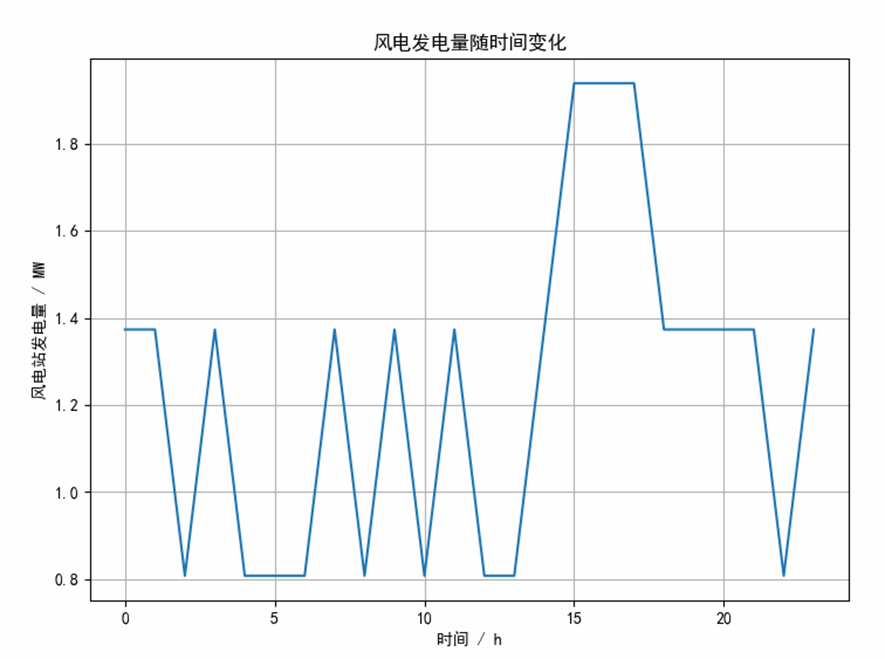
\includegraphics[width=0.9\linewidth]{pictures/screenshot019}
			\label{fig9a}   %以pic.jpg的0.5倍大小输出
		\end{minipage}
	}
	\subfigure[某日0-24时海上风力发电机组输出功率(标幺值)] %第一张子图
	{
		\begin{minipage}{0.5\linewidth}
			\centering          %子图居中
			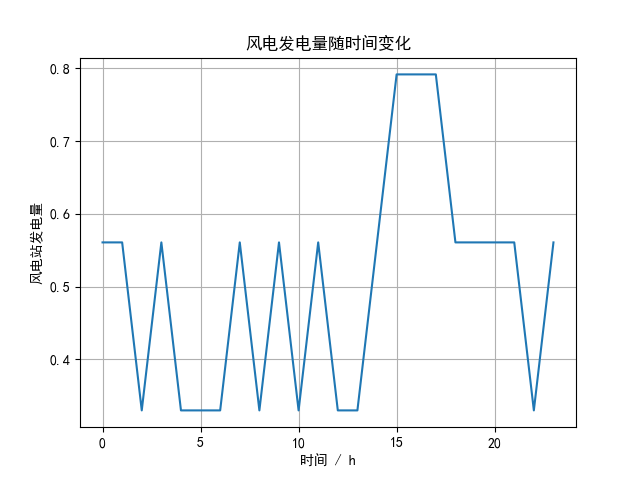
\includegraphics[width=0.9\linewidth]{pictures/screenshot018}
			\label{fig9b}   %以pic.jpg的0.5倍大小输出
		\end{minipage}
	}
	\caption{风电站} %  %大图名称
	\label{fig:9}  %图片引用标记
\end{figure}

电动机$ M1,M2 $和$ M3 $所输入的电能比分别为$ 32.24\%,33.06\% $和$ 34.7\% $,图\ref{fig10a}和\ref{fig10b}分别为3台电动机输入功率的有名值图和标幺值图(基准值分别为$ 0.79MW,0.81M $W和$ 0.84MW $)。\\
\begin{figure}[ht]
	\subfigure[某日0-24时三台电动机输入功率(有名值)] %第一张子图
	{
		\begin{minipage}{0.5\linewidth}
			\centering          %子图居中
			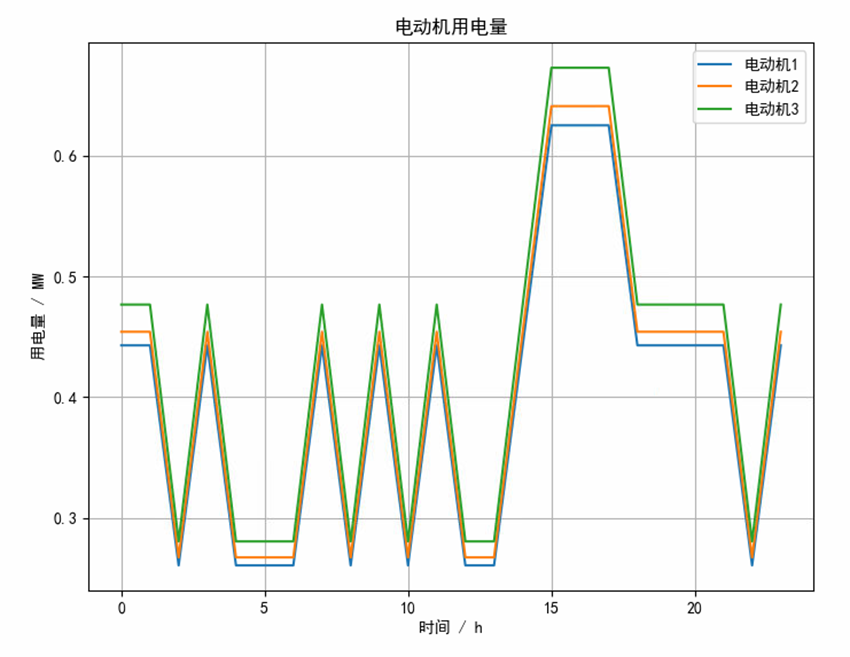
\includegraphics[width=0.9\linewidth]{pictures/screenshot020}
			\label{fig10a}   %以pic.jpg的0.5倍大小输出
		\end{minipage}
	}
	\subfigure[某日0-24时三台电动机输入功率(标幺值)] %第一张子图
	{
		\begin{minipage}{0.5\linewidth}
			\centering          %子图居中
			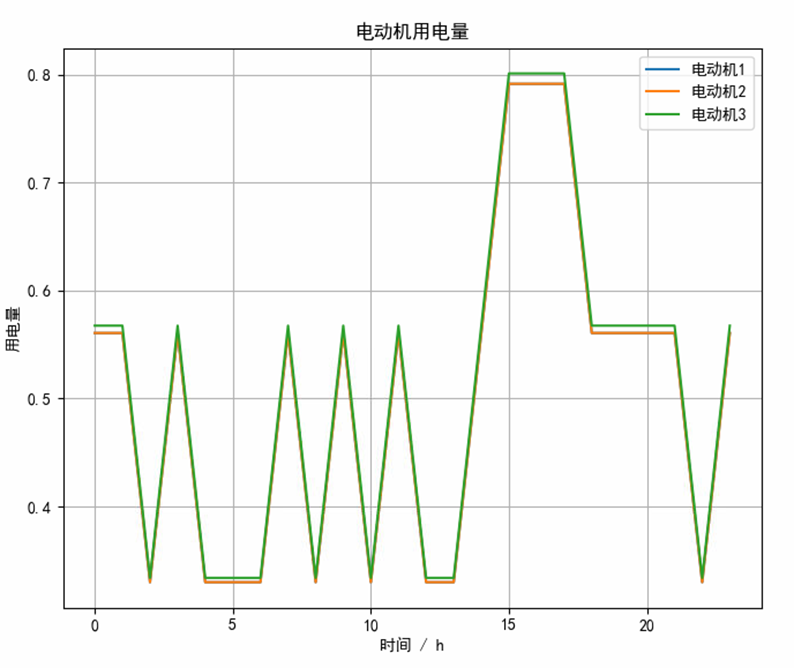
\includegraphics[width=0.9\linewidth]{pictures/screenshot021}
			\label{fig10b}   %以pic.jpg的0.5倍大小输出
		\end{minipage}
	}
	\caption{电动机} %  %大图名称
	\label{fig:10}  %图片引用标记
\end{figure}

电动机$ M1,M2 $和$ M3 $驱动空气压缩机$ C1,C2 $和$ C3 $对空气进行三级压缩,因电动机输入功率随时间变化,故进入压缩机的空气质量流量也随时间变化,图\ref{fig11a}和图\ref{fig11b}所示分别为空气质量流量随时间变化的标幺值图(基准值为$ 8.5kg/s $)和有名值图。\\
\begin{figure}[ht]
	\subfigure[某日0-24时空气质量流量变化(有名值)] %第一张子图
	{
		\begin{minipage}{0.5\linewidth}
			\centering          %子图居中
			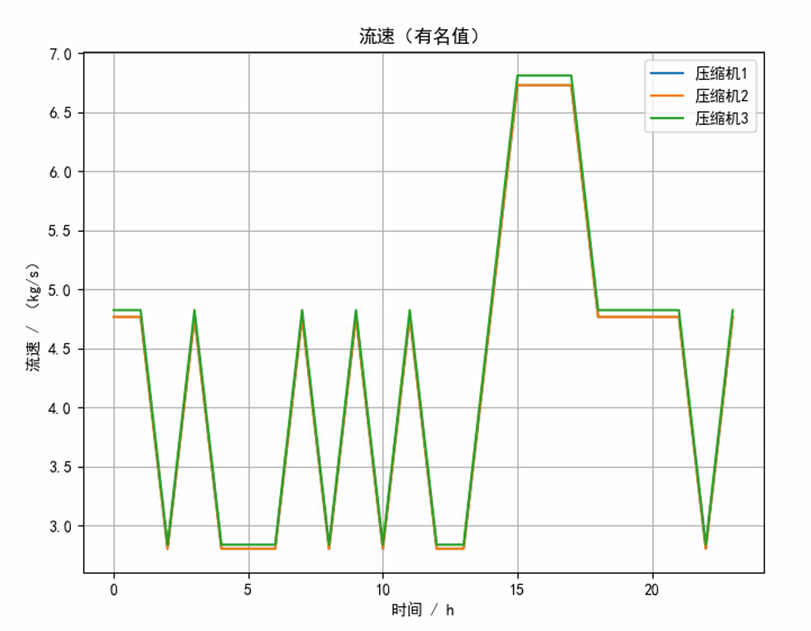
\includegraphics[width=0.9\linewidth]{pictures/screenshot022}
			\label{fig11a}   %以pic.jpg的0.5倍大小输出
		\end{minipage}
	}
	\subfigure[某日0-24时空气质量流量变化(标幺值)] %第一张子图
	{
		\begin{minipage}{0.5\linewidth}
			\centering          %子图居中
			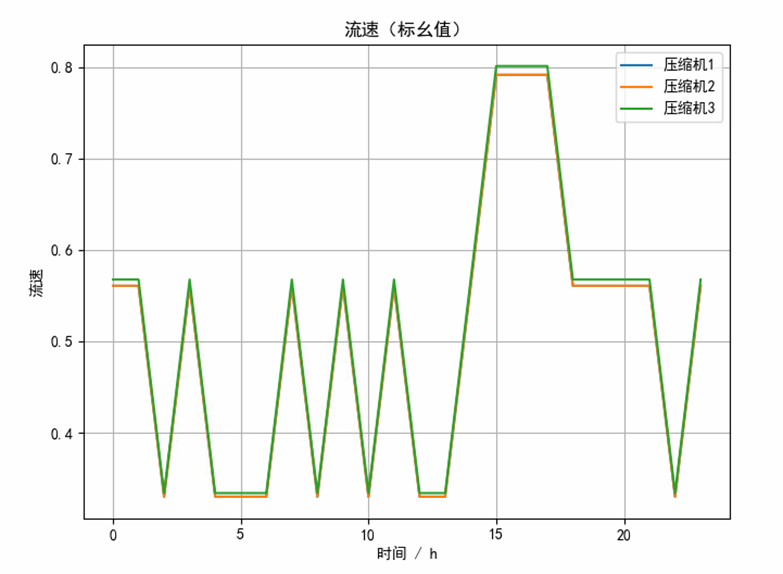
\includegraphics[width=0.9\linewidth]{pictures/screenshot023}
			\label{fig11b}   %以pic.jpg的0.5倍大小输出
		\end{minipage}
	}
	\caption{空气质量流量} %  %大图名称
	\label{fig:11}  %图片引用标记
\end{figure}

如图\ref{fig12a}因受空气质量流量变化的影响,故三台压缩机的压缩效率也表现为随时间变化,压缩效率变化,进而导致压缩终温和高温导热油温度变化。
\begin{figure}[h]
	\centering
	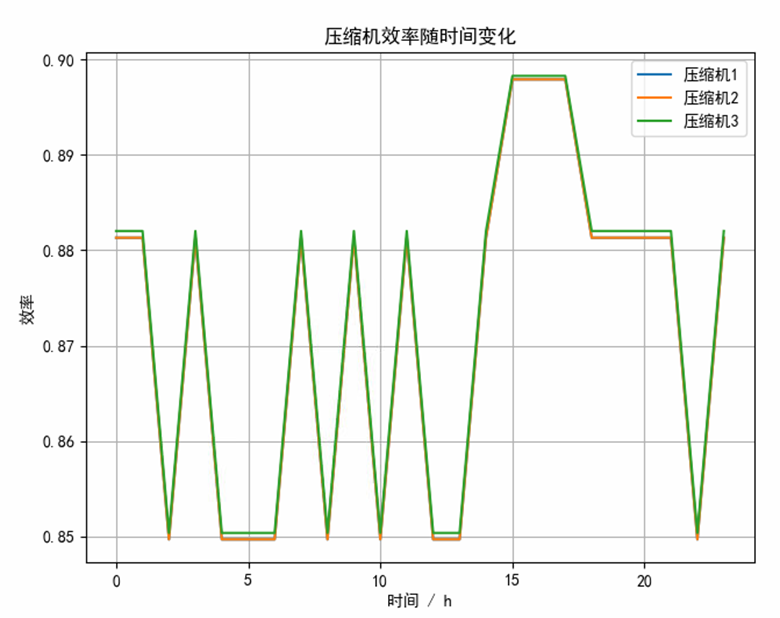
\includegraphics[width=0.7\linewidth]{pictures/screenshot024}
	\caption{某日0-24时三台压缩机压缩效率变化}
	\label{fig12a}
\end{figure}

将图\ref{fig9a}风电站输出功率和图\ref{fig11a}空气质量流量分别对时间积分,得到如图\ref{fig12b}所示的海上风力发电机组总发电量与时间的关系图和图\ref{fig12c}所示的储气包储存空气总质量与时间的关系图。
\begin{figure}[ht]
	\subfigure[某日0-24时风力发电机组总发电量变化] %第一张子图
	{
		\begin{minipage}{0.5\linewidth}
			\centering          %子图居中
			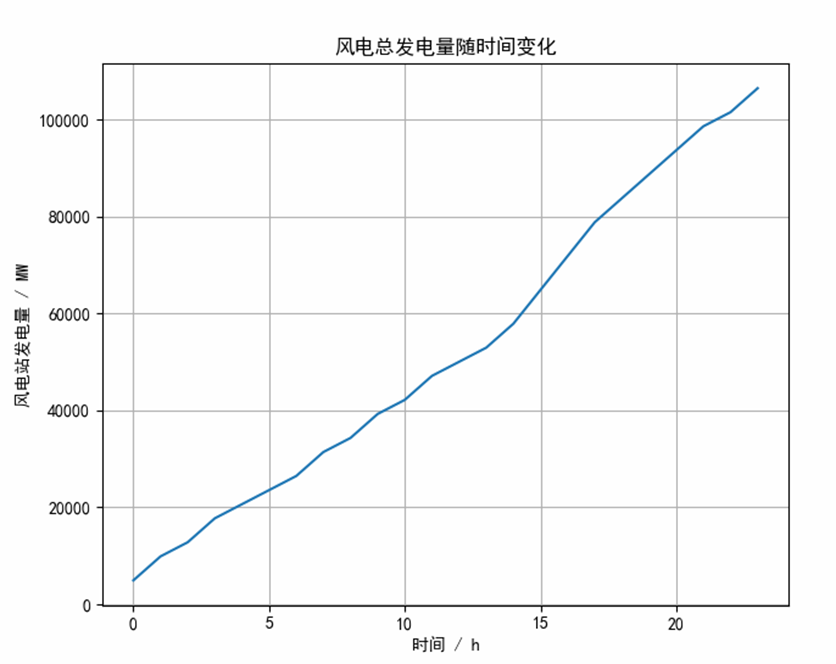
\includegraphics[width=0.9\linewidth]{pictures/screenshot025}
			\label{fig12b}   %以pic.jpg的0.5倍大小输出
		\end{minipage}
	}
	\subfigure[某日0-24时储气包内压缩空气总质量变化] %第一张子图
{
	\begin{minipage}{0.5\linewidth}
		\centering          %子图居中
		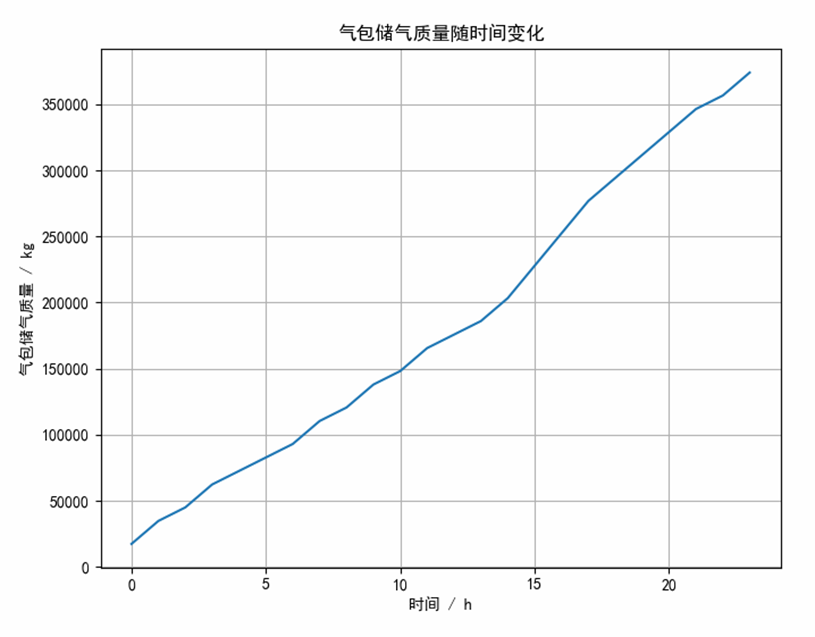
\includegraphics[width=0.9\linewidth]{pictures/screenshot026}
		\label{fig12c}   %以pic.jpg的0.5倍大小输出
	\end{minipage}
}
	\caption{积分结果} %  %大图名称
	\label{fig:13}  %图片引用标记
\end{figure}

根据数据统计,工业用电和居民用电高峰期为每日$ 18:00-23:00 $,因此规定本系统压缩储能时段为每日$ 0:00-15:00 $,高压空气存储时段为每日$ 15:00-18:00 $,膨胀释能时段为每日$ 18:00-20:30 $。这样规定的目的是在非用电高峰期进行压缩储能,用电高峰期膨胀释能来使得本系统输出的电能最大化地被利用,减轻其它常规发电机构的负荷。每日$ 15:00-18:00 $位高压空气储存阶段,该阶段内储气包空气气压损失忽略不计,每日$ 18:00-20:30 $为膨胀释能时段,膨胀释能过程运行在系统设计工况条件下,图4.19所示为储存高压空气时段和膨胀释能时段储气包内空气质量变化与时间的关系图,图4.20所示为膨胀释能时段发电机$ G1,G2,G3 $输出功率与时间的关系图。综合上述分析,可得表\ref{tab:my-table2}所示的各时段相关参数。根据表\ref{tab:my-table2}数据和式\ref{f33}可得,系统效率$ \eta_{system}=\frac{48060}{69652} \times 100\%=69\% $。

\begin{figure}[ht]
	\subfigure[储存空气和膨胀释能时段储气包内压缩空气总质量变化] %第一张子图
	{
		\begin{minipage}{0.5\linewidth}
			\centering          %子图居中
			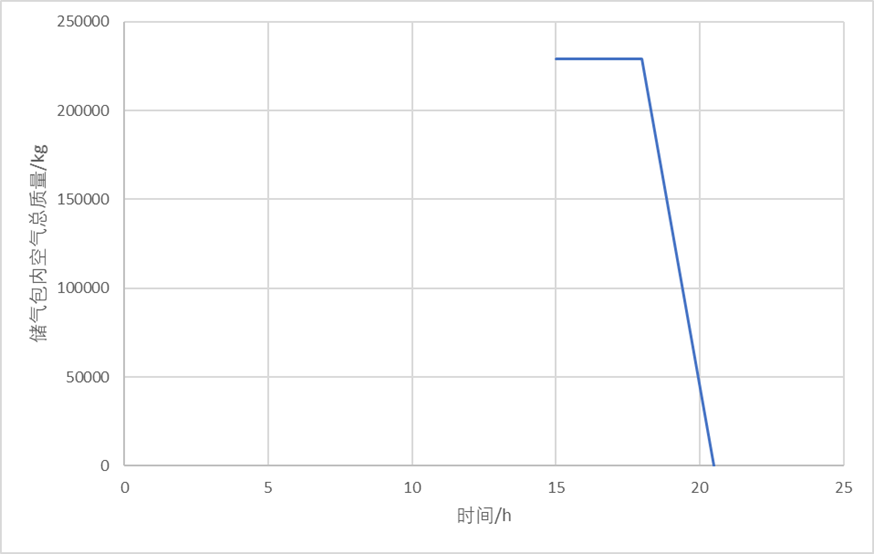
\includegraphics[width=0.9\linewidth]{pictures/screenshot027}
			\label{fig14a}   %以pic.jpg的0.5倍大小输出
		\end{minipage}
	}
	\subfigure[膨胀释能时段三台发电机输出功率变化] %第一张子图
	{
		\begin{minipage}{0.5\linewidth}
			\centering          %子图居中
			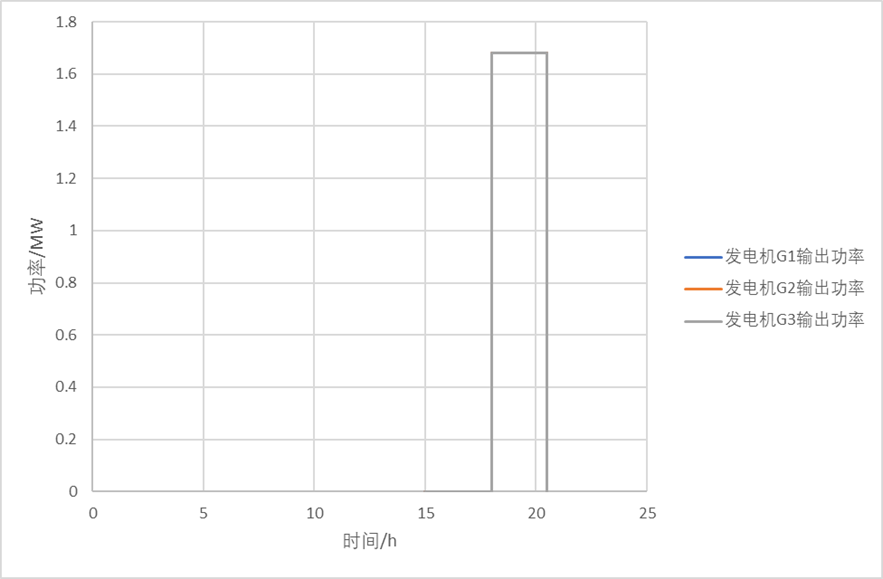
\includegraphics[width=0.9\linewidth]{pictures/screenshot028}
			\label{fig14b}   %以pic.jpg的0.5倍大小输出
		\end{minipage}
	}
	\caption{膨胀过程} %  %大图名称
	\label{fig:14}  %图片引用标记
\end{figure}

\begin{table}[h]
	\resizebox{\textwidth}{!}{
\begin{tabular}{|c|c|r|r|r|r|r|r|}
	\hline
	\multicolumn{1}{|l|}{过程} & \multicolumn{1}{l|}{时段} & \multicolumn{1}{l|}{本时段海上风力}  & \multicolumn{1}{l|}{储气包储气} & \multicolumn{1}{l|}{发电机G1} & \multicolumn{1}{l|}{发电机G2} & \multicolumn{1}{l|}{发电机G3} & \multicolumn{1}{l|}{本时段内发电机}     \\
	\multicolumn{1}{|l|}{}   & \multicolumn{1}{l|}{}   & \multicolumn{1}{l|}{发电机组总发电量} & \multicolumn{1}{l|}{总质量}   & \multicolumn{1}{l|}{输出功率}  & \multicolumn{1}{l|}{输出功率}  & \multicolumn{1}{l|}{输出功率}  & \multicolumn{1}{l|}{G1G2G3输出总电能} \\ \hline
	压缩储能                     & 0:00-15:00              & 69652MW                       & 229500kg                   & 0                          & 0                          & 0                          & 0                                \\ \hline
	储存空气                     & 15:00-18:00             & 0                             & 229500kg                   & 0                          & 0                          & 0                          & 0                                \\ \hline
	膨胀时能                     & 18:00-20:30             & 0                             &                            & 1.78MW                     & 1.78MW                     & 1.78MW                     & 48060MW                          \\ \hline
\end{tabular}
}
	\caption{系统变工况条件下运行各时段发电量}
	\label{tab:my-table2}
\end{table}

\newpage
\section{系统经济效益分析}\ \\

根据4.2.2变工况实例分析结果,本节主要是对海上风力发电-水下压缩空气储能互补系统进行长远性的经济效益分析,并以此作为该系统可行性的重要依据。\\

首先讨论系统运行的成本问题。本系统所需成本主要由4个方面组成:
\begin{enumerate}
	\item 系统部件购买成本
	\item 系统部件安装成本
	\item 系统部件维护保养成本
	\item 系统部件故障维修成本
\end{enumerate}

依据当前机械市场数据,其具体所需金额如表\ref{tab:my-table5}所示。因为该系统是关系到国民经济发展的能源系统,故系统所有部件划分为特种机械范畴,根据《TSG特种设备安全技术规范》规定,系统自运行起每月需进行一次维护保养,其费用约为24980元/整系统次。至于故障维修成本是这样规定的,根据特种设备月故障次数函数拟合图\ref{fig15a}所示,计算出如图\ref{fig15b}所示的日故障概率图,并在系统模型中调用随机函数随机得出设备在规定运行年限内的故障次数,并规定故障维修费用为48400元/次。\\

% Please add the following required packages to your document preamble:
% \usepackage{multirow}
% \usepackage{graphicx}
\begin{table}[h]
	\resizebox{\textwidth}{!}{
		\begin{tabular}{|l|r|r|r|r|c|c|}
			\hline
			\multicolumn{1}{|c|}{环节} &
			\multicolumn{1}{c|}{所需容量} &
			\multicolumn{1}{c|}{单价} &
			\multicolumn{1}{c|}{成本/元} &
			\multicolumn{1}{c|}{安装费用/元} &
			维护保养费用/(元/整系统·次) &
			故障维修费用/(元/次) \\ \hline
			风力发电机 &
			5MW &
			1000元/kW &
			5000000 &
			500000 &
			{}{}{24980} &
			{}{}{48600} \\ \cline{1-5}
			电动机M1   & 1MW     & 200元/kW   & 200000   & 20000   &  &  \\ \cline{1-5}
			电动机M2   & 1MW     & 200元/kW   & 200000   & 20000   &  &  \\ \cline{1-5}
			电动机M3   & 1MW     & 200元/kW   & 200000   & 20000   &  &  \\ \cline{1-5}
			空气压缩机1  & 1MW     & 600元/kW   & 600000   & 60000   &  &  \\ \cline{1-5}
			空气压缩机2  & 1MW     & 600元/kW   & 600000   & 60000   &  &  \\ \cline{1-5}
			空气压缩机3  & 1MW     & 600元/kW   & 600000   & 60000   &  &  \\ \cline{1-5}
			空气膨胀机1  & 2MW     & 600元/kW   & 1200000  & 120000  &  &  \\ \cline{1-5}
			空气膨胀机2  & 2MW     & 600元/kW   & 1200000  & 120000  &  &  \\ \cline{1-5}
			空气膨胀机3  & 2MW     & 600元/kW   & 1200000  & 120000  &  &  \\ \cline{1-5}
			发电机G1   & 2MW     & 500元/kW   & 1000000  & 100000  &  &  \\ \cline{1-5}
			发电机G2   & 2MW     & 500元/kW   & 1000000  & 100000  &  &  \\ \cline{1-5}
			发电机G3   & 2MW     & 500元/kW   & 1000000  & 100000  &  &  \\ \cline{1-5}
			换热器1    & -       & 100000元/台 & 100000   & 10000   &  &  \\ \cline{1-5}
			换热器2    & -       & 100000元/台 & 100000   & 10000   &  &  \\ \cline{1-5}
			换热器3    & -       & 100000元/台 & 100000   & 10000   &  &  \\ \cline{1-5}
			换热器4    & -       & 100000元/台 & 100000   & 10000   &  &  \\ \cline{1-5}
			换热器5    & -       & 100000元/台 & 100000   & 10000   &  &  \\ \cline{1-5}
			换热器6    & -       & 100000元/台 & 100000   & 10000   &  &  \\ \cline{1-5}
			柔性储气包   & 30000m³ & 300元/m³   & 9000000  & 900000  &  &  \\ \cline{1-5}
			管路,线路连接 & -       & -         & 1760000  & 23600   &  &  \\ \cline{1-5}
			热液罐     & -       & 100000元/个 & 100000   & 10000   &  &  \\ \cline{1-5}
			冷液罐     & -       & 100000元/个 & 100000   & 10000   &  &  \\ \cline{1-5}
			合计      & -       & -         & 25560000 & 2403600 &  &  \\ \hline
		\end{tabular}
	}
	\caption{系统运行成本}
	\label{tab:my-table5}
\end{table}
\begin{figure}[ht]
	\subfigure[特种设备月故障次数函数拟合图] %第一张子图
	{
		\begin{minipage}{0.5\linewidth}
			\centering          %子图居中
			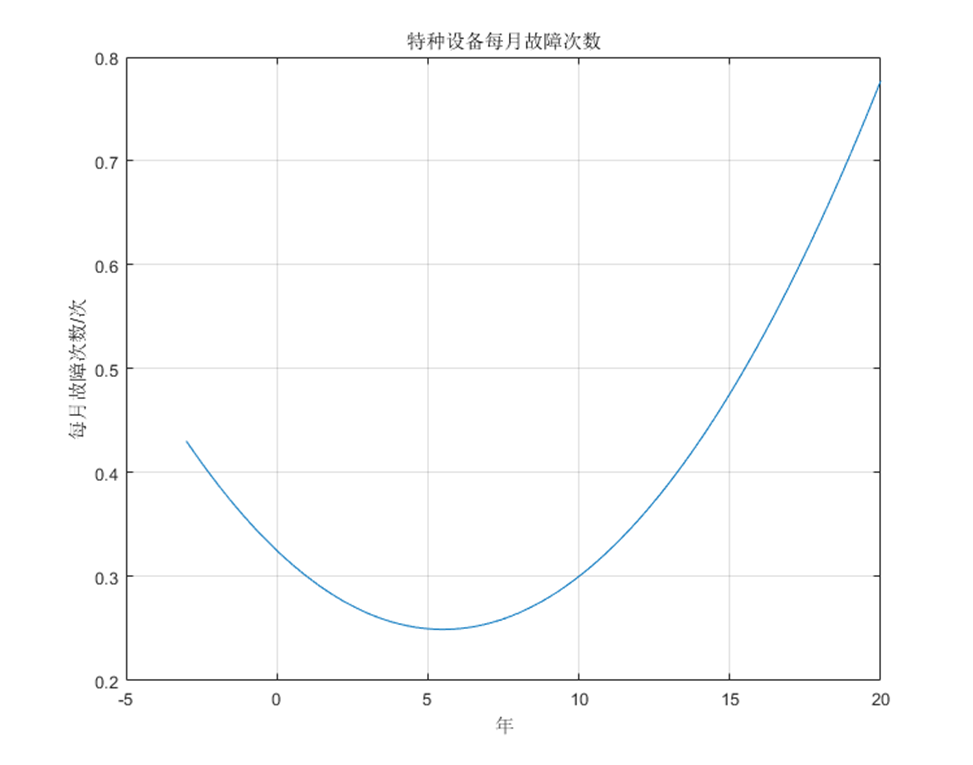
\includegraphics[width=0.9\linewidth]{pictures/screenshot029}
			\label{fig15a}   %以pic.jpg的0.5倍大小输出
		\end{minipage}
	}
	\subfigure[特种设备日故障概率图] %第一张子图
	{
		\begin{minipage}{0.5\linewidth}
			\centering          %子图居中
			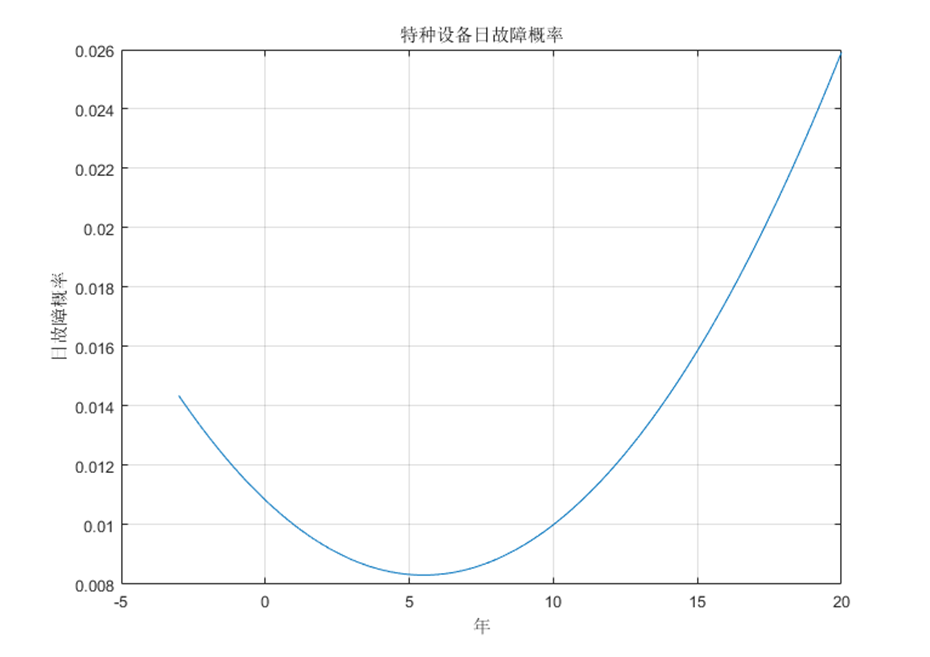
\includegraphics[width=0.9\linewidth]{pictures/screenshot030}
			\label{fig15b}   %以pic.jpg的0.5倍大小输出
		\end{minipage}
	}
	\caption{特种设备日故障次数及概率} %  %大图名称
	\label{fig:15}  %图片引用标记
\end{figure}



\begin{table}[ht]
	\centering
	\resizebox{0.5\textwidth}{!}{
	\begin{tabular}{|l|r|r|}
		\hline
		用电类型                       & \multicolumn{1}{l|}{用电比例} & \multicolumn{1}{l|}{单价/(元/KWh)} \\ \hline
		工业用电                       & 78\%                      & 0.62                            \\ \hline
		\multicolumn{1}{|c|}{居民用电} & 22\%                      & 1.025                           \\ \hline
	\end{tabular}
}
	\caption{18:00-20:30用电类型占比及单价}
	\label{tab:my-table3}
\end{table}

% Please add the following required packages to your document preamble:
% \usepackage{graphicx}
\newpage
\begin{table}[ht]
	\centering
	\resizebox{0.8\textwidth}{!}{%
		\begin{tabular}{|l|l|l|l|l|l|}
			\hline
			\begin{tabular}[c]{@{}l@{}}发电总\\ 功率/kW\end{tabular} &
			\begin{tabular}[c]{@{}l@{}}日发电\\ 时长/h\end{tabular} &
			\begin{tabular}[c]{@{}l@{}}日发电\\ 量/kWh\end{tabular} &
			\begin{tabular}[c]{@{}l@{}}工业用电\\ 收入/(元/日)\end{tabular} &
			\begin{tabular}[c]{@{}l@{}}居民用电\\ 收入/(元/日)\end{tabular} &
			收入/(元/日) \\ \hline
			\multicolumn{1}{|r|}{5040} &
			\multicolumn{1}{r|}{2.5} &
			\multicolumn{1}{r|}{12600} &
			\multicolumn{1}{r|}{9326} &
			\multicolumn{1}{r|}{2630} &
			\multicolumn{1}{r|}{11865} \\ \hline
		\end{tabular}%
	}
	\caption{系统无故障条件下的日发电量及日收入}
	\label{tab:my-table4}
\end{table}

其次讨论系统运行的收入问题,根据参考文献\cite{b4}得知本系统的发电时段18:00-20:30所处的用电高峰期内居民用电占比约为22\%,工业用电占比为78\%,珠海市电单价如表\ref{tab:my-table3}所示。参考表\ref{tab:my-table2}数据,可得表\ref{tab:my-table4}所示的系统无故障条件下的日发电量及日收入数据。并规定若当日系统发生故障,并且当日无收入。\\

将成本计算方法和日收入计算方法输入到系统模型中,得到如图\ref{fig:screenshot031}所示的系统运行成本、总收入、净收入变化图。通过观察图\ref{fig:screenshot031},发现系统运行月9.58年时,开始盈利,在特种机械有效寿命20内,总净收入可达2.81千万元。

\begin{figure}[ht]
	\centering
	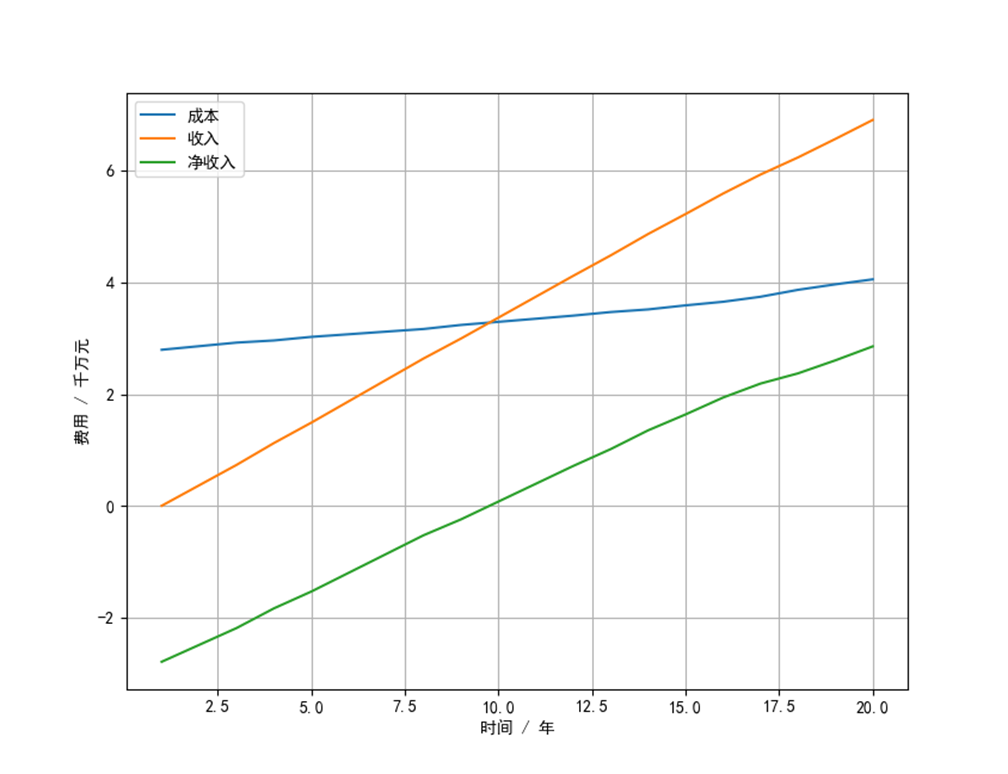
\includegraphics[width=0.7\linewidth]{pictures/screenshot031}
	\caption{系统运行成本、总收入、净收入变化}
	\label{fig:screenshot031}
\end{figure}
\newpage
\section{结论}\ \\

本文围绕所设计的海上风力发电-水下压缩空气储能互补系统进行能效分析和经济效益分析,综合考虑了该新能源系统的能源利用有效性、经济性和可实现性等多方面问题。系统模型的仿真结果显示,借助海上风力发电机组、空气压缩机、柔性储气包、空气膨胀机、换热器等主要机械部件构成的海上风力发电-水下压缩空气互补系统可以将随机性强波动性大的海上风能先转化为稳定的物质内能,再转化为稳定输出的电能,实现了能量从不稳定输出到稳定输出的转变,相比于传统的风力发电,大大减小了能源系统输出电能对电网的冲击,保障了电网、国民经济生产和人民生活用电的安全。同时,将柔性储气包设置在海洋100m左右的环境时,在风速随机波动条件下系统效率仍可达69\%,且安装难度较小和安装成本较低,整个系统在有效寿命20期限内可获得近2.85千万元的总利润,做到了系统能效性和经济性的统一,为系统的可实现性提供了重要依据,供相关能源部门决策参考。


\newpage
\begin{thebibliography}{100}
%引用用\cite
 \bibitem{b5}
贾涛,王兴月. \emph{海洋平台多能互补系统电源容量优化}. [J].\hskip 1em plus
0.5em minus 0.4em\relax 太重(天津)滨海重型机械有限公司技术中心. 2017. 

 \bibitem{b4}
李建民. \emph{夏季用电高峰期间电气设备运行重点}. [J].\hskip 1em plus
0.5em minus 0.4em\relax 北京电力亦庄供电公司. 2006. 

\bibitem{b1}
王志文. \emph{水下压缩空气储能系统设计与能效分析}. [D].\hskip 1em plus
0.5em minus 0.4em\relax 大连海事大学. 2017.

\bibitem{b2}
王志文,熊伟,王海涛,王祖温. \emph{水下压缩空气储能研究进展}. [J].\hskip 1em plus
0.5em minus 0.4em\relax 大连海事大学船舶机电装备研究所. 2015.

\bibitem{b8}
闫晔. \emph{考虑风电不确定性的分时电价研究}. [D].\hskip 1em plus
  0.5em minus 0.4em\relax 西安理工大学. 2020.
  
  \bibitem{b6}
  Brian C. Cheung, Rupp Carriveau, David S.K. Ting. \emph{Multi-objective optimization of an underwater compressed air energy
  	storage system using genetic algorithm}. [J].\hskip 1em plus
  0.5em minus 0.4em\relax Turbulence and Energy Laboratory, Ed Lumley Centre for Engineering Innovation, University of Windsor. 2014. 
  
   \bibitem{b7}
  F. Fornarelli, S.M. Camporeale, B. Fortunato, M. Torresi, P. Oresta, L. Magliocchetti, A. Miliozzi,
  G. Santo
  . \emph{CFD analysis of melting process in a shell-and-tube latent heat storage
  	for concentrated solar power plants}. [J].\hskip 1em plus
  0.5em minus 0.4em\relax a Politecnico di Bari, Dipartimento di Ingegneria Meccanica, Matematica e Management, Sezione di Macchine ed Energetica, Via Orabona 4, 70125 Bari, Italy. 2016. 
  
\bibitem{b3}
Wolf D. \emph{Methods for Design and Application of Adiabatic Compressed Air Energy Storage Based on Dynamic Modeling}. [D].\hskip 1em plus
0.5em minus 0.4em\relax Ruhr-Universitat Bochum. 2010. 





\end{thebibliography}
%\end{multicols}



 \end{document}